
%----------------------------------------------------------------------------------------
%	4./ Data reduction
%----------------------------------------------------------------------------------------
%\label{se:dataproc}

The raw KID data ($I$, $Q$, $\Delta I$, $\Delta Q$) and the telescope
source-tracking data are synchronized by the NIKA2 acquisition system using a
clock that gives the absolute astronomical time, that is the telescope
pulses per second, to define the NIKA2 raw data. From the KID raw
data, we compute a quantity that is proportional to the KID
frequency shift using the \emph{RfdIdQ} method, as described in
Sect.~\ref{se:tuning}. This quantity, which is hence proportional to
the input signal, constitutes the KID time-ordered information (TOI).

%For each observing scan, NIKA2 produce a datastream via the data
%acquisition software, which synchronises with the telescope data using
%pulses per second (pps). This clock is itself synchronous to the
%absolute astronomical time. Using the \rf\ photometric
%estimator, as discussed in Sect.~\ref{se:tuning}, we derive the
%timelines of the KID resonance frequency estimate, which is a quantity
%proportionnal to the flux absorbed by a KID and
%homogeneous to Hz~\citep[see]{Calvo2013}. These time ordered
%information (TOI), together with
%the time-stamped pointing information produced by the telescope,
%constitute the raw data.

We have developed a dedicated data reduction pipeline to
produce calibrated sky maps from NIKA2 raw data. This pipeline was first 
developed for the data analysis during the commissioning campaigns and
is currently used for science-purpose data reduction. The calibration
and performance assessment relies on this pipeline. 
A detailed description of this software will be presented in a companion
paper \citep{Ponthieu2019}, as well as an application to blind source
detection. Here we summarize the main steps of the data
reduction. {\lp Moreover, we focus the discussion on the treatment of
point-like or compact sources, which are used for the
performance assessment.}

%\section{Data Reduction}
%\label{se:dataproc}
%
%Because each matrix of \nika\ is a filled array with more than one
%detector per \new{main beam} PSF on average, and because the atmosphere and electronic noise act as
%correlated low frequency parasites, the data reduction of \nika\ does not
%proceed on an individual KID basis in general. This, in addition to the
%necessary pointing information specifies some of the data reduction
%process. In short, the data reduction proceeds as such:
%
%\begin{itemize}
%\item Low level processing (Sect.~\ref{se:ll_proc})
%\item Pointing reconstruction (Sect.~\ref{se:ptg})
%\item TOI calibration and opacity correction (Sect.~\ref{se:flux_calib})
%\item TOI processing (Sect.~\ref{se:toi_proc})
%\item Map projection (Sect.~\ref{se:map_projection})
%\item Photometry (Sect.~\ref{se:intro_photometry})
%\end{itemize}

%\noindent{\emph{Low level processing:}
%\paragraph{Low level processing.}
\subsection{Low level processing}
\label{se:ll_proc}
%A first step of the analysis is to read the data produced by \nika's
%acquisition. The data as such comprise various quantities that describe the
%variations of the KID's resonance frequencies, such as $I$, $Q$, $dI$,
%$dQ$. From these quantities, and throughout this work, we use our so called
%\rf\ photometric estimator that combines them into a quantity that is
%proportionnal to the flux absorbed by a KID \citep[see]{Calvo2013} and
%homogeneous to Hz, as discussed in Sect.~\ref{se:tuning}.
We isolate the relevant fraction of the data for scientific
utilisation and {\lp we mask KIDs that do not meet the selection criteria, as
discussed in Sect.~\ref{se:avg_kidpar},} or
timeline accidents (glitches). Specifically, we flag out cosmic rays,
which impact only one data sample per hit due to the KID fast time
constant~\citep{Catalano2014}, %periods
%dedicated to the KID resonance frequency {\tt tuning}
%(Sect.~\ref{se:tuning}),
%of the KID tones to their resonance frequency
and the KIDs for which the noise level exceed $3\sigma$ of the average
noise level of all other KIDs of the same array.  
%In addition to this, we look for and remove the - rare - cosmic rays
%events. KIDs have such fast time constants that unlike bolometers, these events
%affect a sole sample that is easy to detect by a simple comparison to the rms of
%the TOI a few second window. These affected samples are remplaced by a simple
%linear interpolation of their surrounding (not to leave holes in the TOI) but
%are flagged in order not to project false data on the final map.
%
%We also have a series of tests that read the flags produced by the acquisition
%overall: discontinuity in the temperature within the cryostat as well
%as detector tuning that automatically trigger at the beginning and the
%end of each scans are discarded.  
%potential jumps in the cryostat or acquisition
%monitoring. Most important are the flags related to the tuning. Because the
%acquisition file boundaries are not strictly linked to the beginning and the end of
%a scan, we must discard everything that happens before the last tuning of the
%beginning, and everything after the first automatic tuning that happens when the
%scan is done.
%
%Because the tuning of KIDs might fail from time to time depending on the weather
%conditions for instance, we systematically check each KID and see if its noise
%is far from the average noise of all other KIDs in the same array, with a
%typical $3\,\sigma$ threshold. This criterion may seem a bit tight, but in any case, KIDs
%are inverse noise variance weighted in the final map projection, so they would
%be given relatively low weight anyway (see Sect.~\ref{se:map_projection}).

%\paragraph{Pointing reconstruction.}
\subsection{Pointing reconstruction}
\label{se:ptg}
We produce a timeline of the pointing positions of each KID with
respect to the targeted source position (usually located at the center of the
scan) using two sets of information. First, the control system of the
telescope provides us with the absolute pointing of a reference point
of the focal point, which is coincident with the reference KID after
the pointing correction are applied, as described in
Sect.~\ref{se:pointing}. Second, we estimate the offset positions of
each KID with respect to the reference KID using a dedicated
procedure that is referred to as the focal plane reconstruction, as
presented in Sect.~\ref{se:geometry}. After this step, we are able to
distinguish KIDs that are on-source from those that are off-source,
which is a key information for dealing with the correlated noise. 
%This step consists in addressing each sample of each KID to the correct sky
%coordinates and their associated map pixel. The pointing data, as
%produced by the control system of the telescope, \aka\ NCS, are passed to the
%\nika\ raw data. They describe the absolute pointing of a reference
%point in the focal plane in various quantities, the
%absolute azimuth and elevation $(\alpha,\delta)$ of the source, together with
%offsets $(\Delta\alpha_t, \Delta\delta_t)$ \wrt~these. Because our final maps
%will be centered on a fixed position (typically the center of the source that is
%aimed by the focal plane reference position), we are especially interested in
%pointing offsets \wrt~this position. We therefore detail here the
%derivation of these offsets.
%
%We store KID pointing offsets \wrt\ the reference position in Nasmyth $(x,y)$
%coordinates (independent of time) once and for all in our KID database
%(\aka~\kidpar). Sect.~\ref{se:geometry} details how these offsets are
%derived. To go from Nasmyth offsets to $(\alpha,\delta)$ offsets, we apply the
%following rotation by the elevation angle:
%
%\begin{eqnarray}
%\Delta\alpha^k_t &=&  \cos\delta_t \Delta x^k + \sin\delta_t \Delta y^k, \nonumber\\
%\Delta\delta^k_t &=& -\sin\delta_t \Delta x^k + \cos\delta_t \Delta y^k, \nonumber
%\end{eqnarray}
%
%where $k$ is a KID index. Adding these offsets to the reference $(\Delta
%\alpha_t, \Delta \delta_t)$ gives the absolute pointing of each KID in these
%coordinates. An extra rotation by the parallactic angle $\eta_t$ is required to
%obtain KID's coordinates in \radec\ coordinates:
%
%\begin{eqnarray}
%\Delta R.\,A.^k_t &=&  \cos\eta_t \Delta\alpha^k_t + \sin\eta_t \Delta\delta^k_t,\\
%\Delta Dec^k_t    &=& -\sin\eta_t \Delta\alpha^k_t + \cos\eta_t \Delta\delta^k_t.
%\end{eqnarray}
%
%We now have the pointing of each KID at each time relative to the source that we
%usually center on our final map. It is then trivial to assign the map pixel
%corresponding to this pointing on a Nearest Grid Point basis.
%
%This pointing reconstruction is done early in the data reduction process because
%we'll need to know when a KID is close or far from the source for the timeline
%processing (Sect.~\ref{se:toi_proc}).\\
  
%\noindent \emph{TOI calibration.}
\subsection{TOI calibration}
\label{se:flux_calib}
The KID TOI in units of Hz (frequency shifts) are converted to
Jy/beam in two steps. First, the KID data are inter-calibrated using the
calibration coefficients, \aka\ relative gains, 
as discussed in Sect.~\ref{se:flat_field} and the
absolute scale of the flux density is set using the absolute
calibration method discussed in
Sect.~\ref{se:calibration_method}. Second, the instantaneous line-of-sight
atmospheric attenuation $\rm{exp}[{-\taunu x(t)}]$ is corrected
using the zenith opacity at the observing frequency $\nu$ $\taunu$, which is estimated for a given scan
as discussed in Sect.~\ref{se:opacity}, and the instantaneous \airmass\
$x(t)$. {\lp The latter is estimated as $(\sin \elev_t)^{-1}$ using the observing elevation
$\elev_t$, as obtained using the pointing reconstruction.}     

%\paragraph{Correlated noise subtraction.}
\subsection{Correlated noise subtraction}
\label{se:toi_proc}
The TOI of each KID include a prominent low-frequency component of correlated noise of two
different origins: the atmospheric component, which is dominant
{\lp with some rare exceptions} and common to all KIDs, and the electronic noise, which is common to the KIDs connected
to a same electronic readout feed-line (see
Sect.~\ref{se:array}). The subtraction of this correlated noise is a key
step of the data processing, as correlated noise residuals are an
important limiting factor of the sensitivity. We have devised several
dedicated methods for this purpose. This will be thoroughly
discussed in \citet{Ponthieu2019}, whereas here we illustrate the
general principle and only discuss the method routinely used for
the calibration.

\begin{figure}[ht!]
\begin{center}
\includegraphics[clip, angle=0, scale=0.4]{Figures/toi_plot.eps}
\includegraphics[clip, angle=0, scale=0.4]{Figures/toi_plot_decorr.eps}
\caption[Example of Time-Ordered-Information]{Example of variations of KID
  time-ordered information. \emph{Top:} Example of 40 KID {\lp calibrated} TOIs during an observation
  of Uranus. The low frequency correlated component (atmospheric and electronic
  noises) is clearly seen. \emph{Bottom:} One of these TOIs (in blue) and the
  \cm\ that is subtracted from it (in red). {\lp The zero level is arbitrary.}}
\label{fig:nika_toi}
\end{center}
\end{figure}

%\begin{figure}[ht!] 
%\begin{center}
%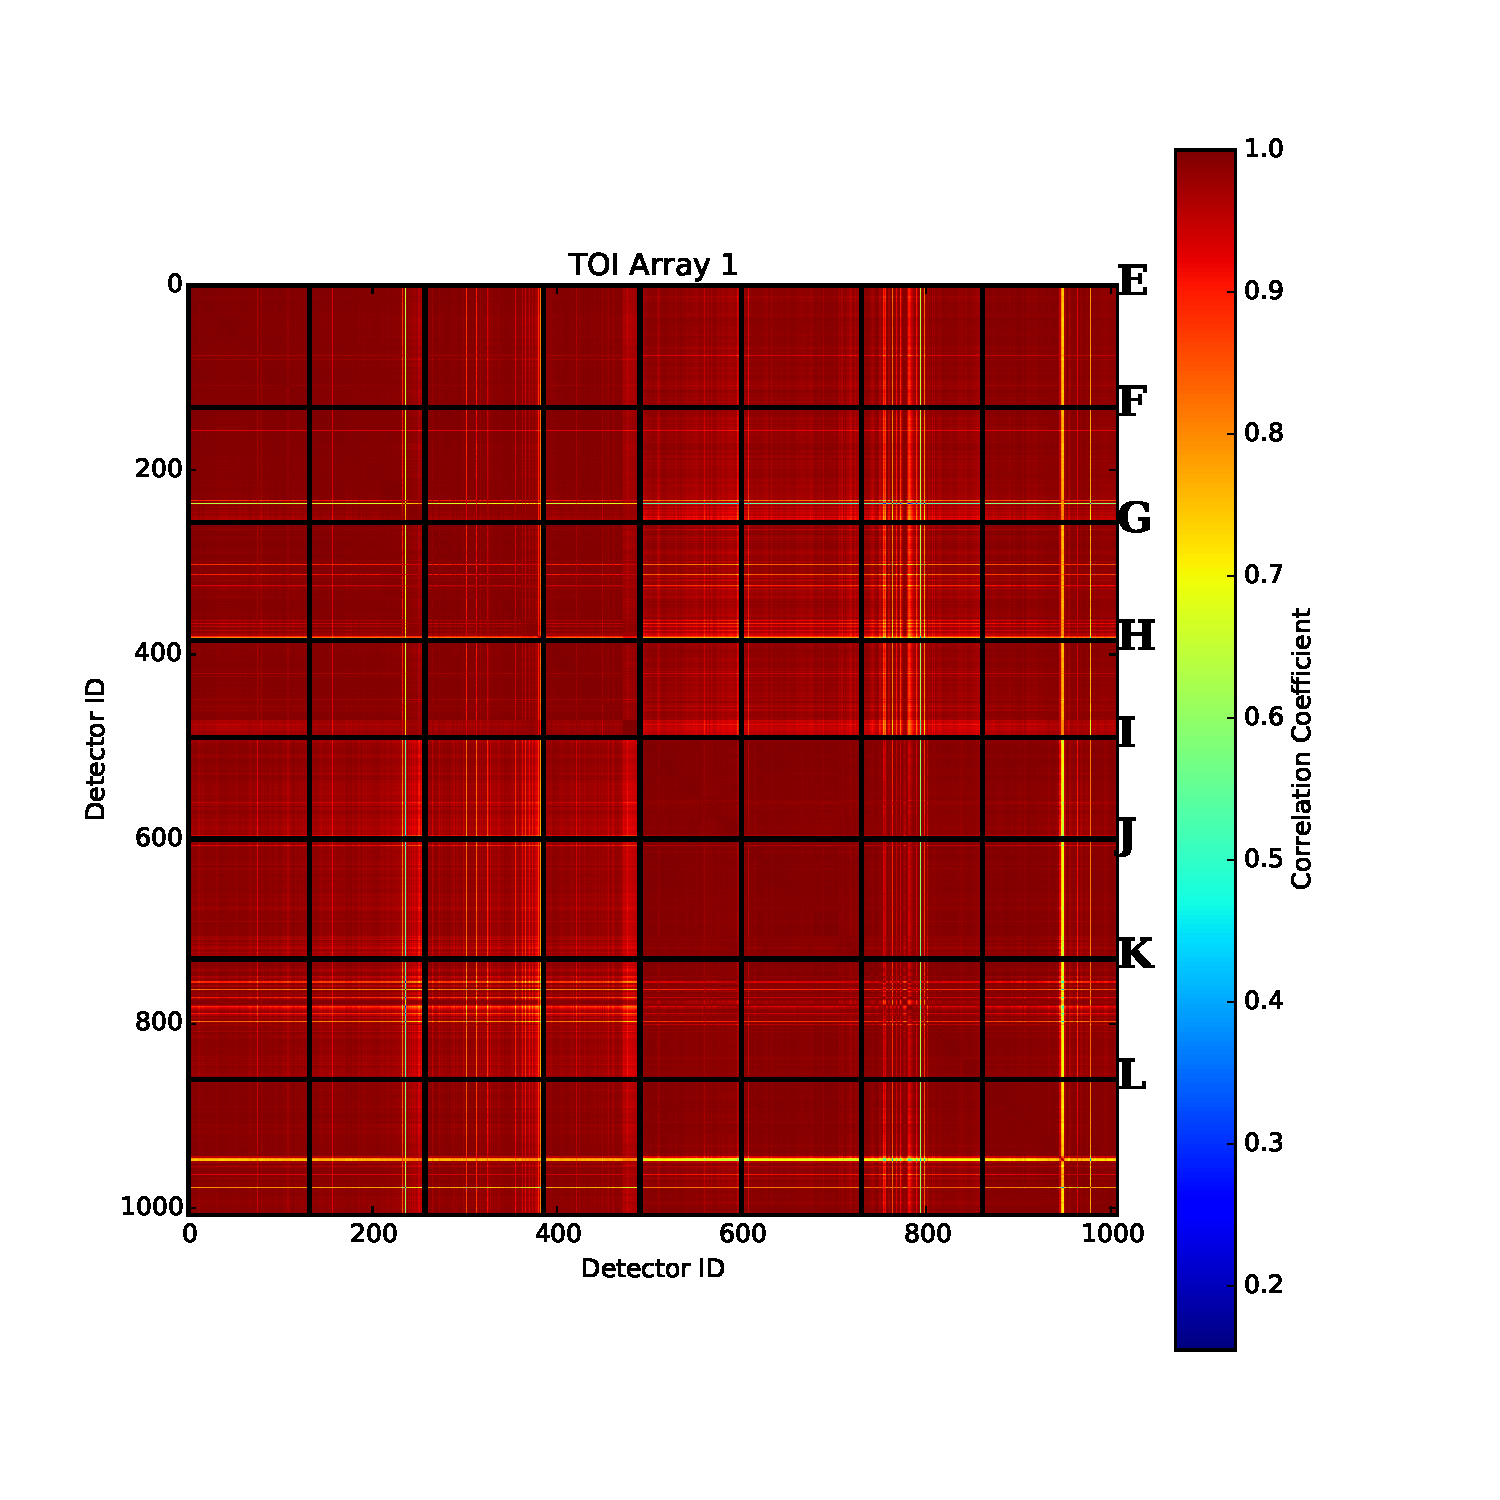
\includegraphics[width=0.3\textwidth]{Figures/NoiseTests/corrmat_TOI_array_1_20170228s151.pdf}
%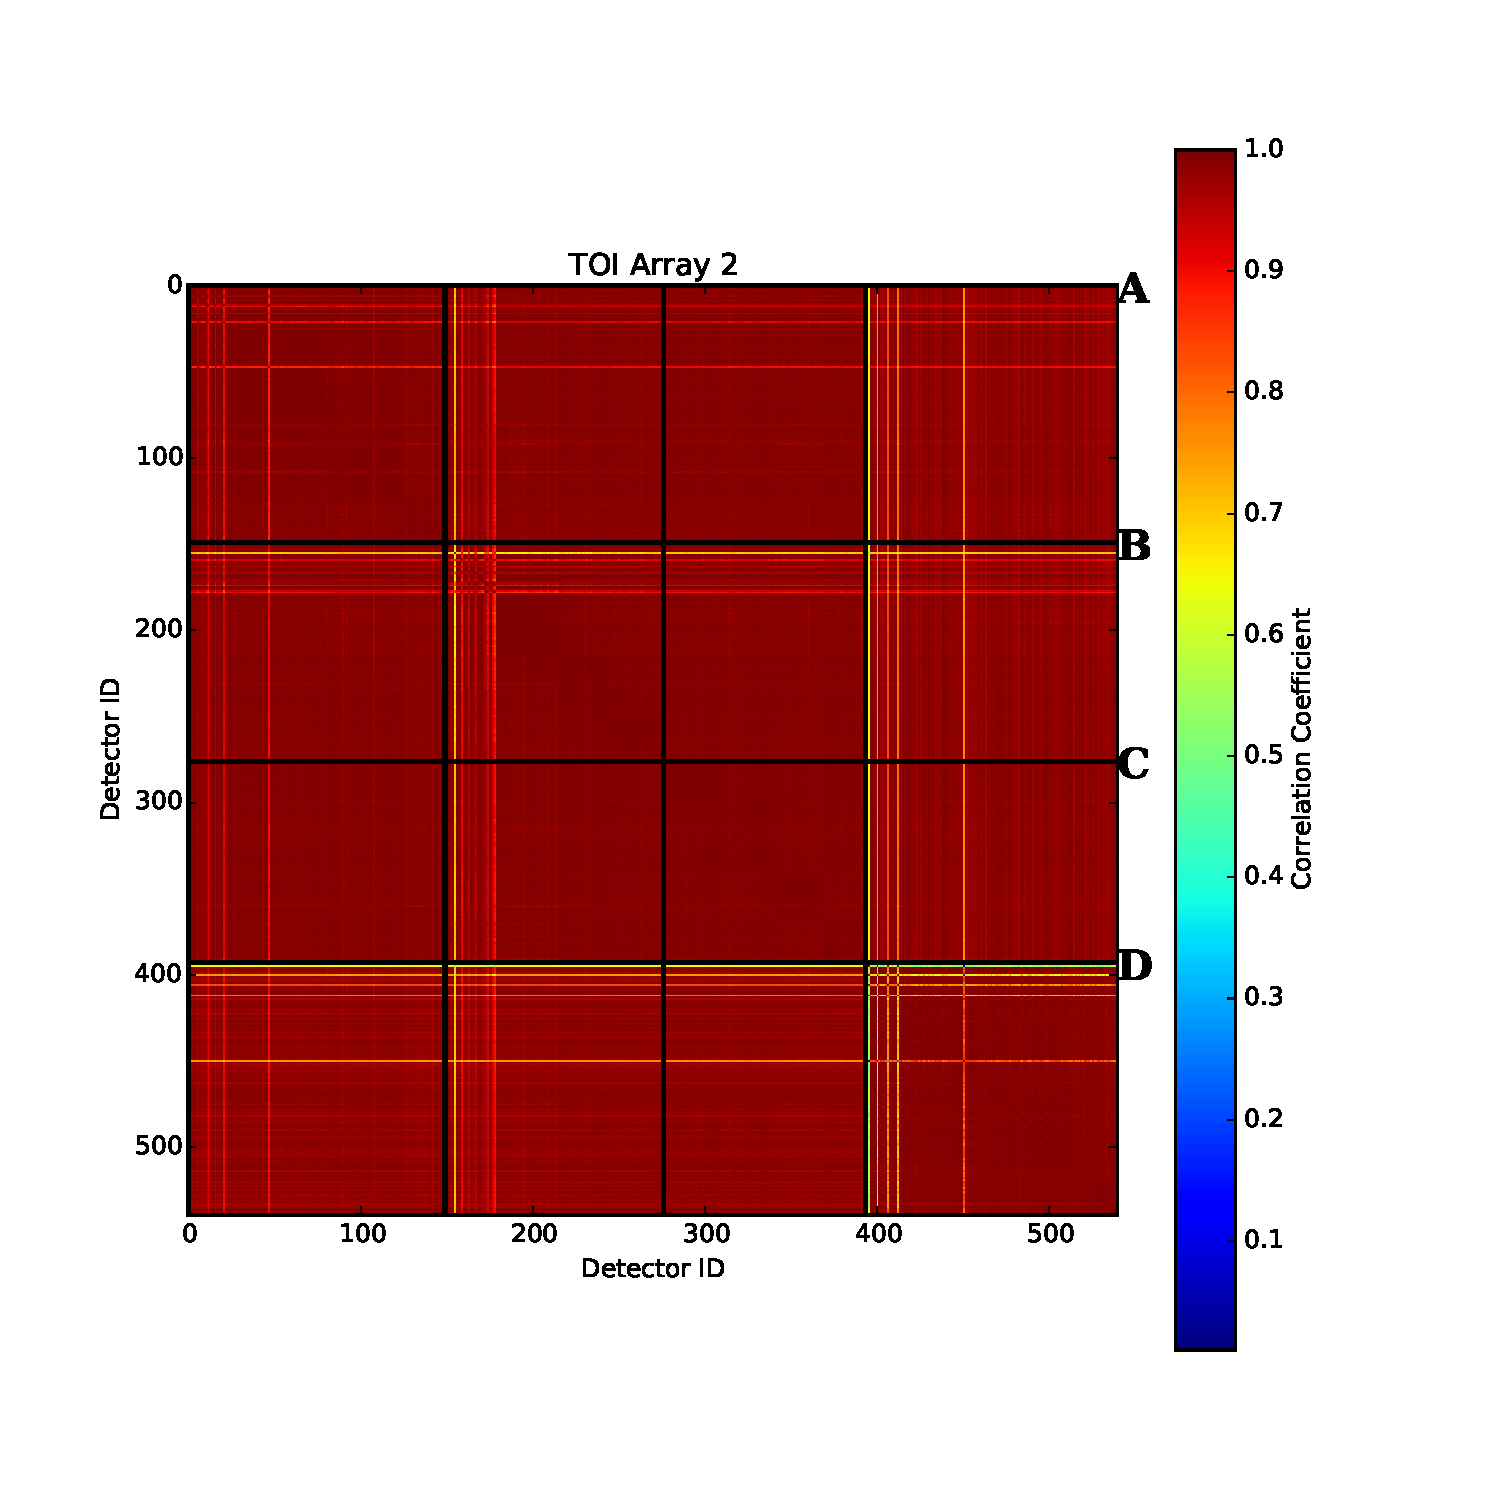
\includegraphics[width=0.3\textwidth]{Figures/NoiseTests/corrmat_TOI_array_2_20170228s151.pdf}
%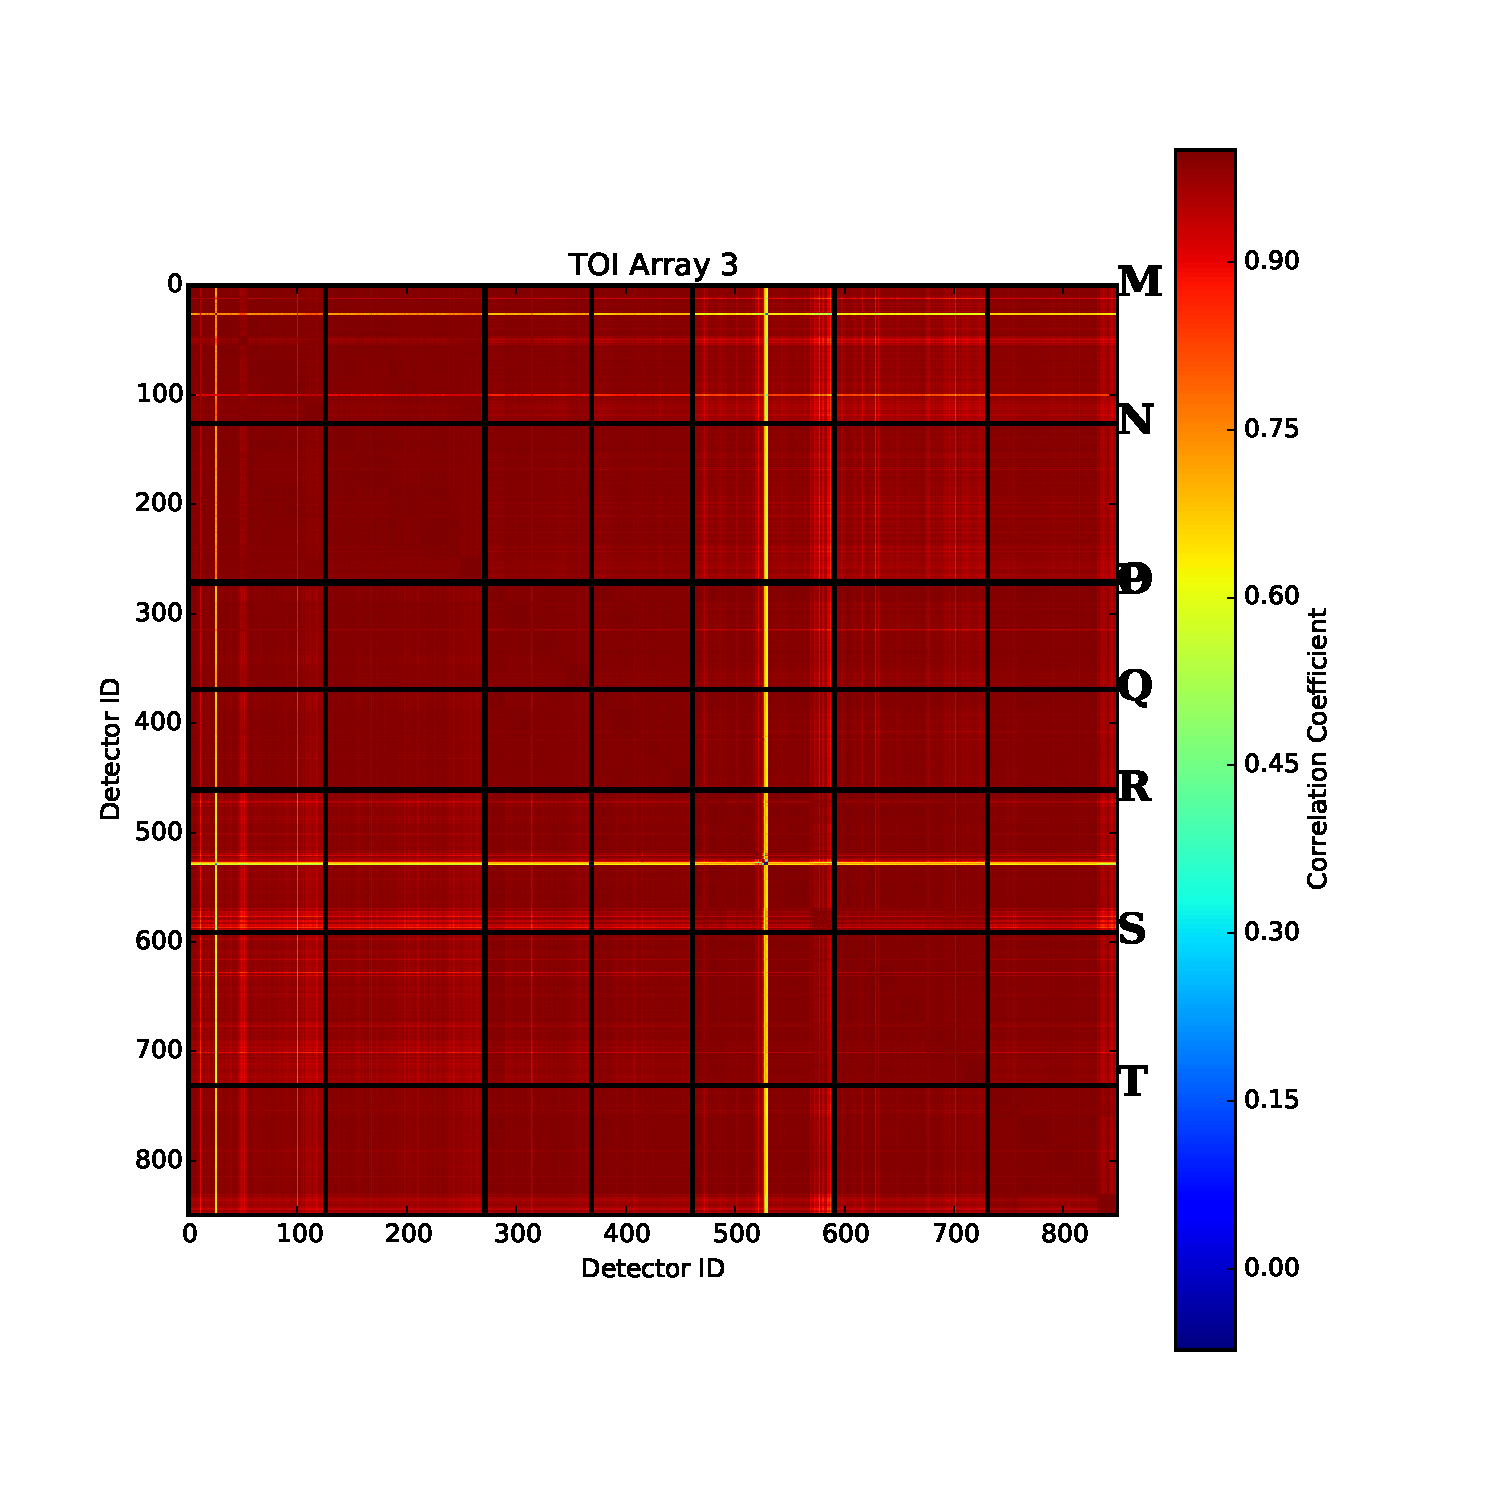
\includegraphics[width=0.3\textwidth]{Figures/NoiseTests/corrmat_TOI_array_3_20170228s151.pdf}
%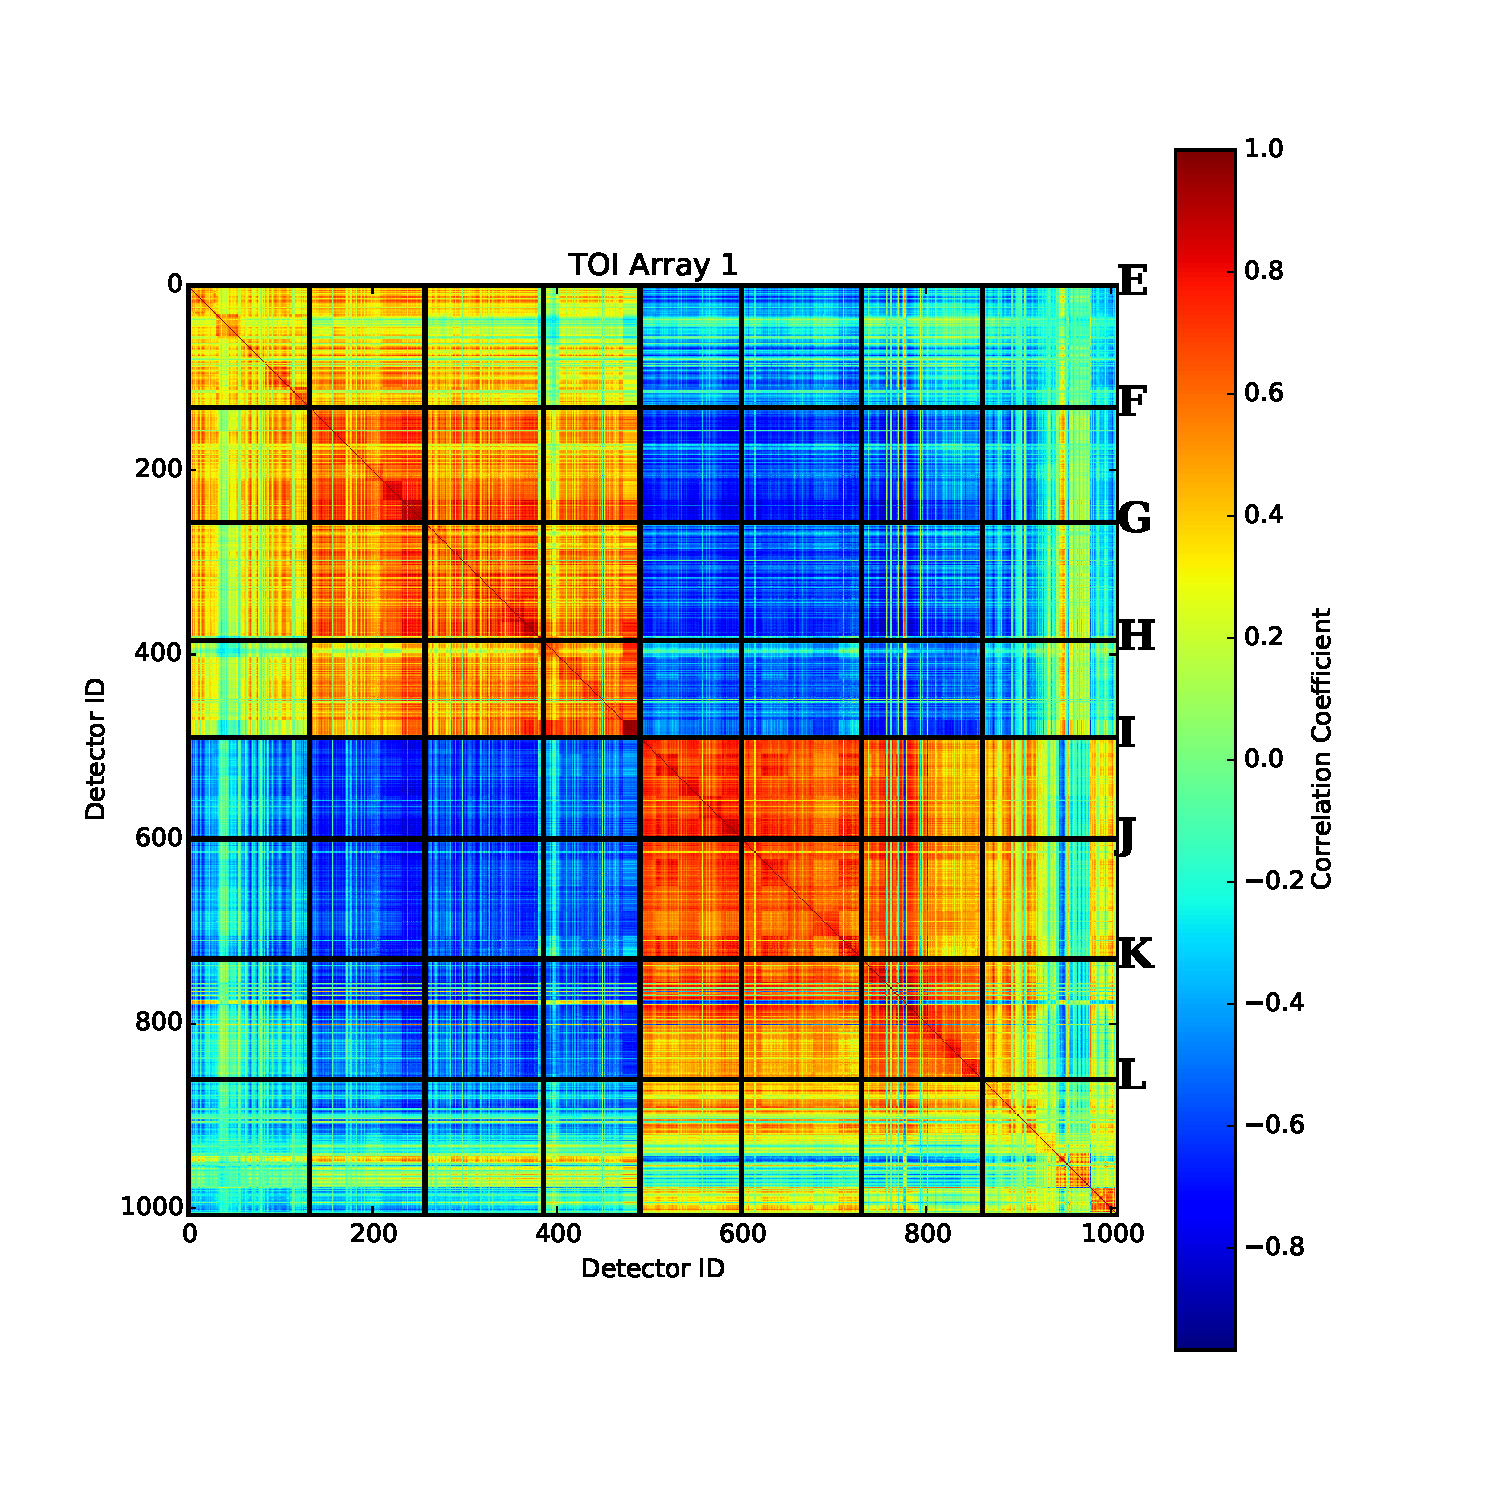
\includegraphics[width=0.3\textwidth]{Figures/NoiseTests/corrmat_TOI_CM_array_1_20170228s151.pdf}
%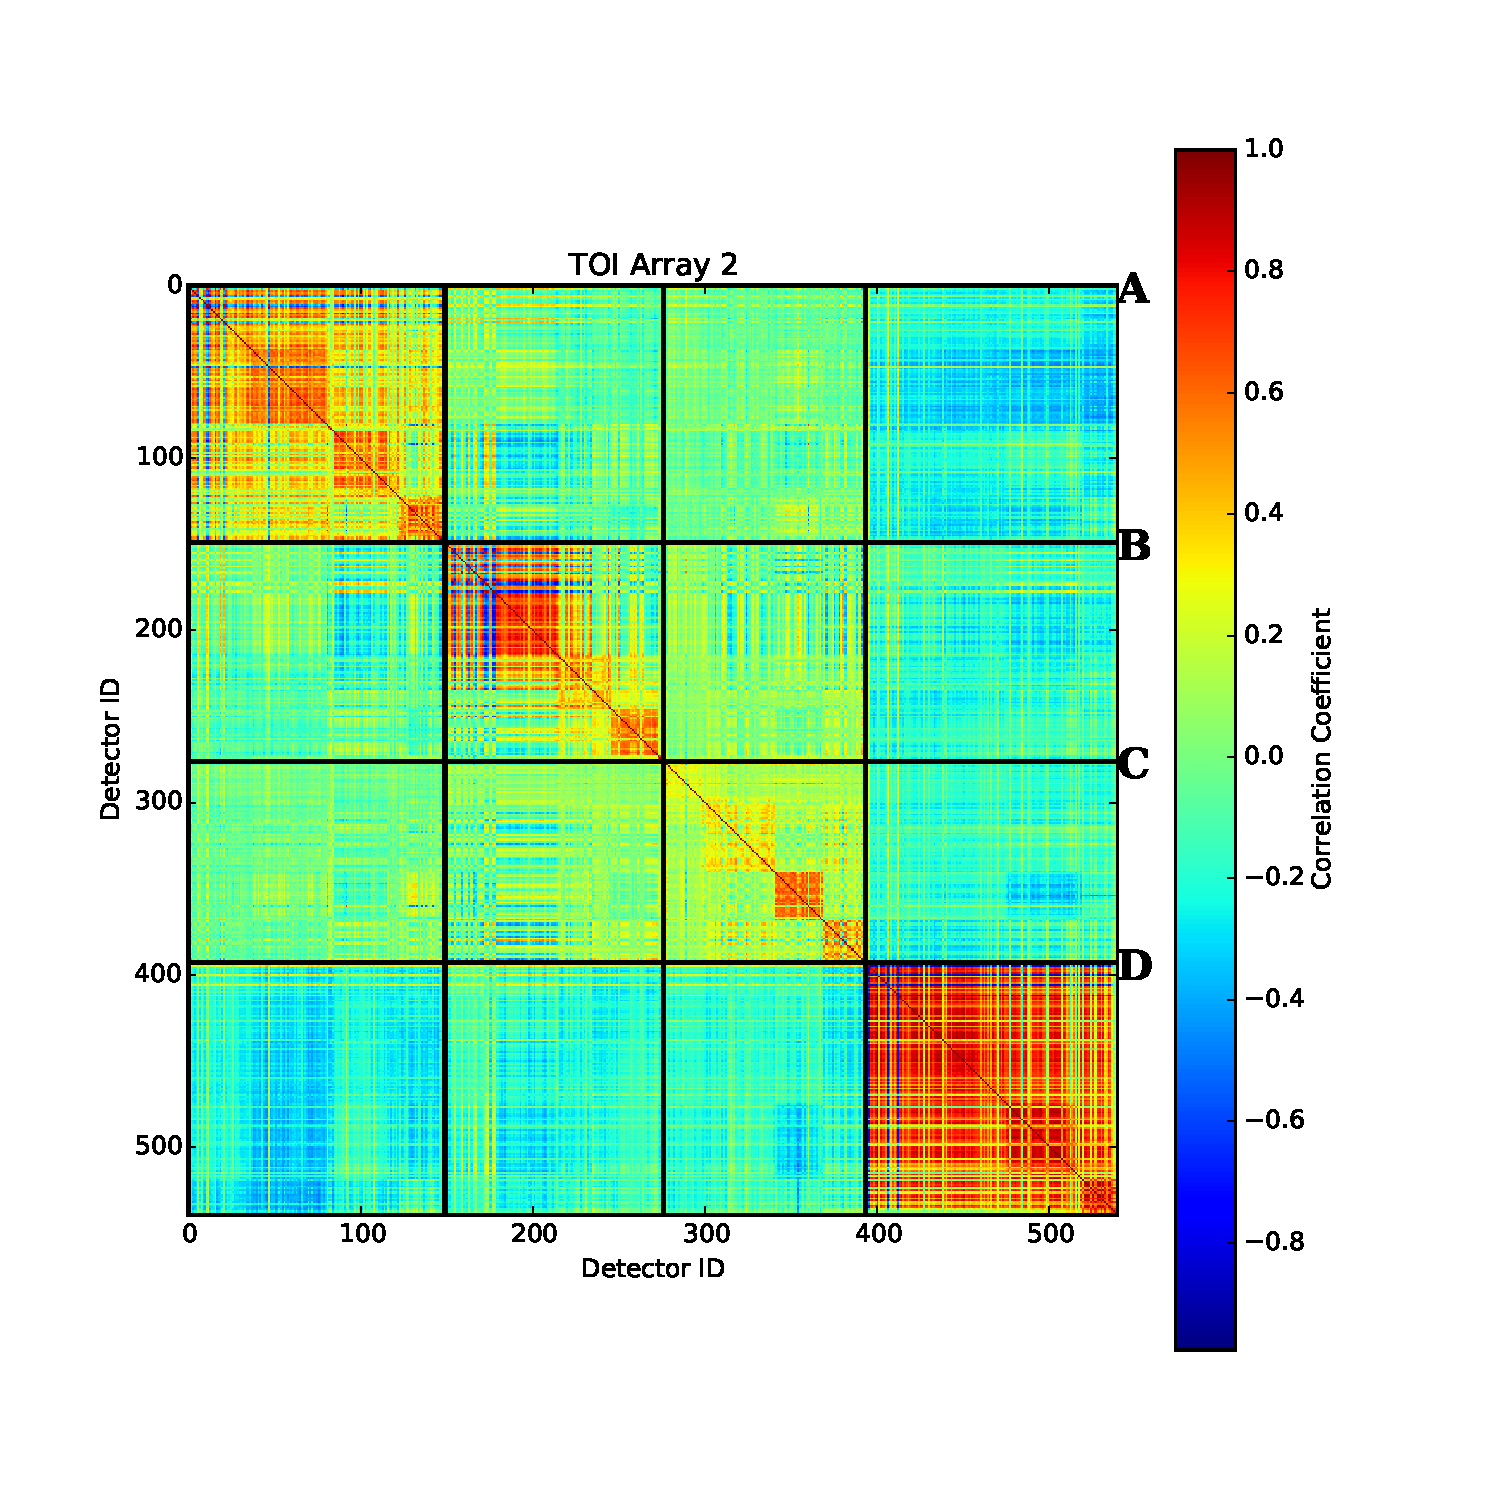
\includegraphics[width=0.3\textwidth]{Figures/NoiseTests/corrmat_TOI_CM_array_2_20170228s151.pdf}
%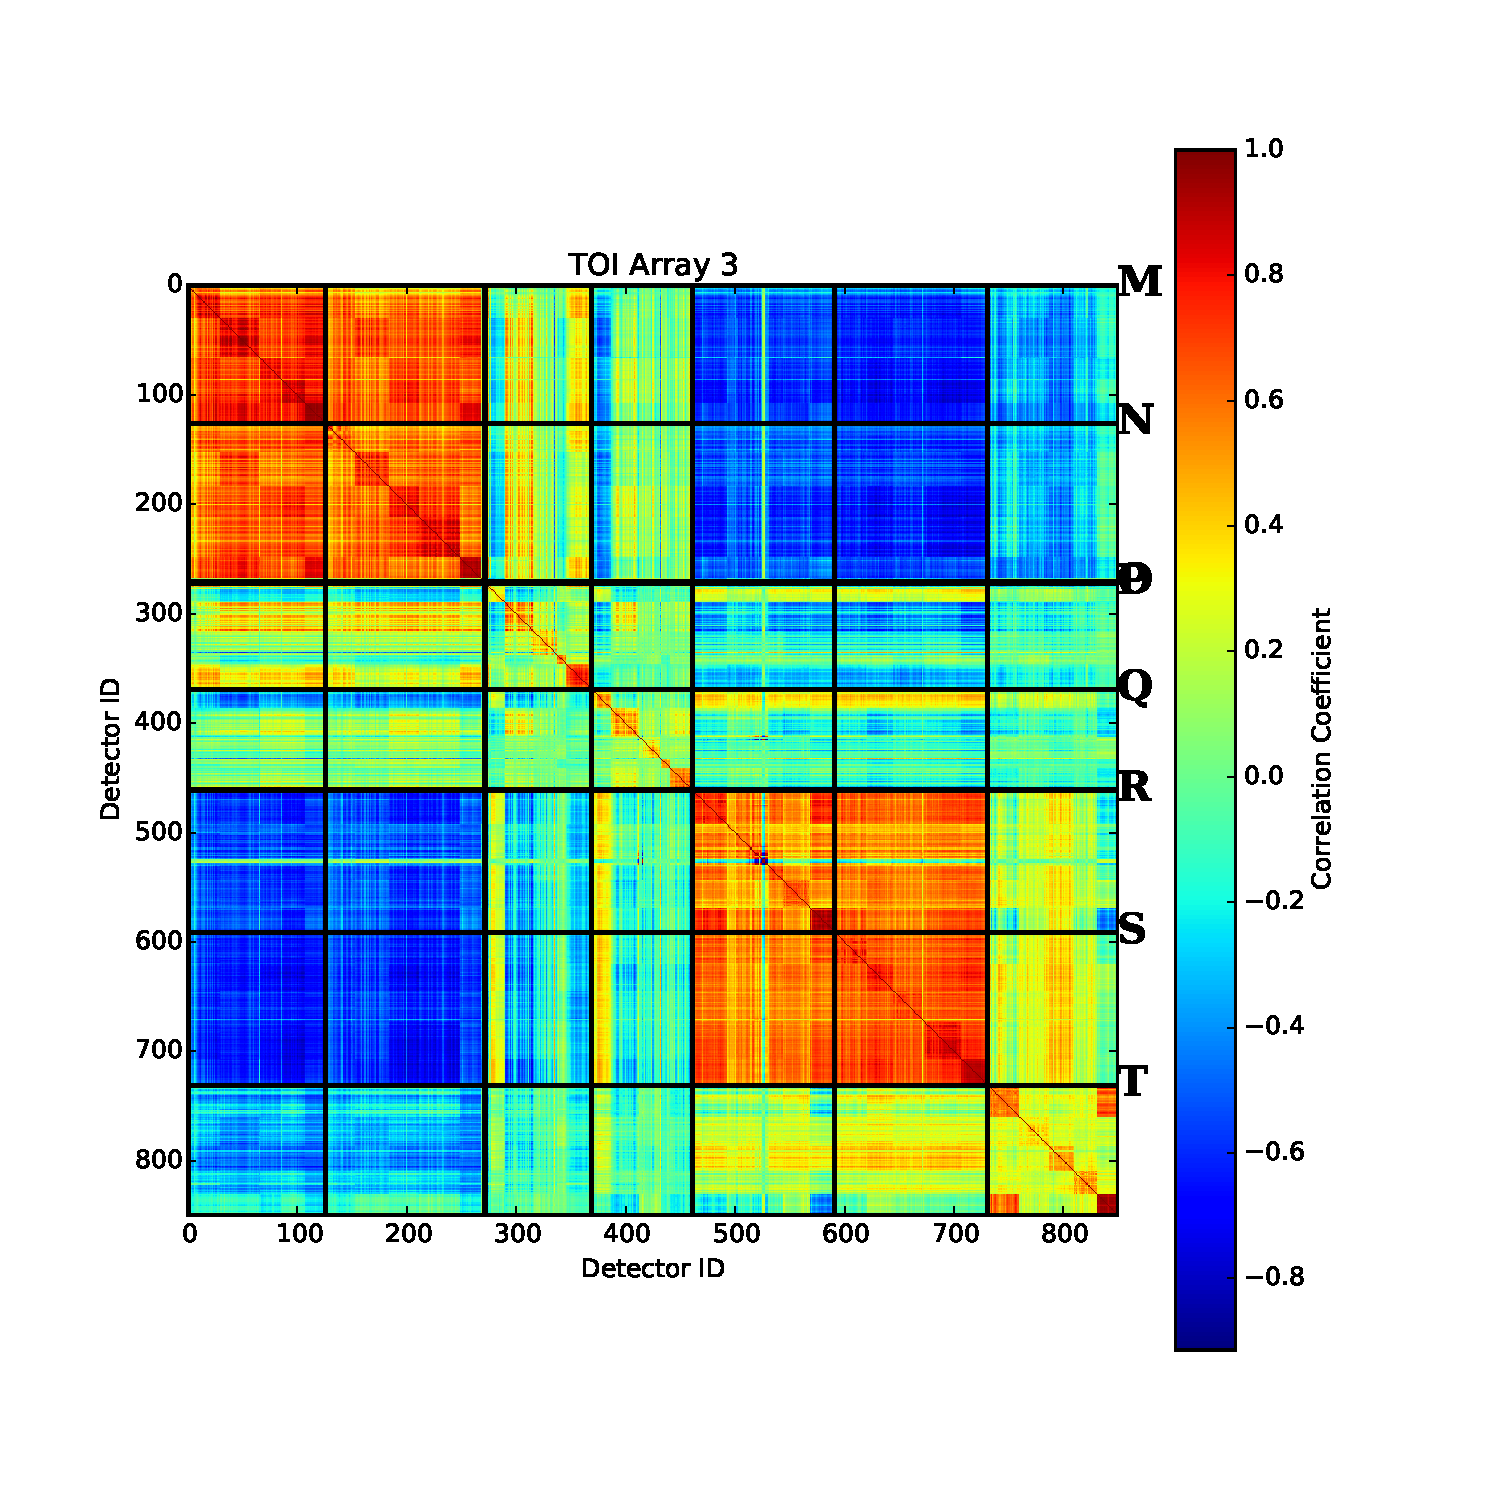
\includegraphics[width=0.3\textwidth]{Figures/NoiseTests/corrmat_TOI_CM_array_3_20170228s151.pdf}
%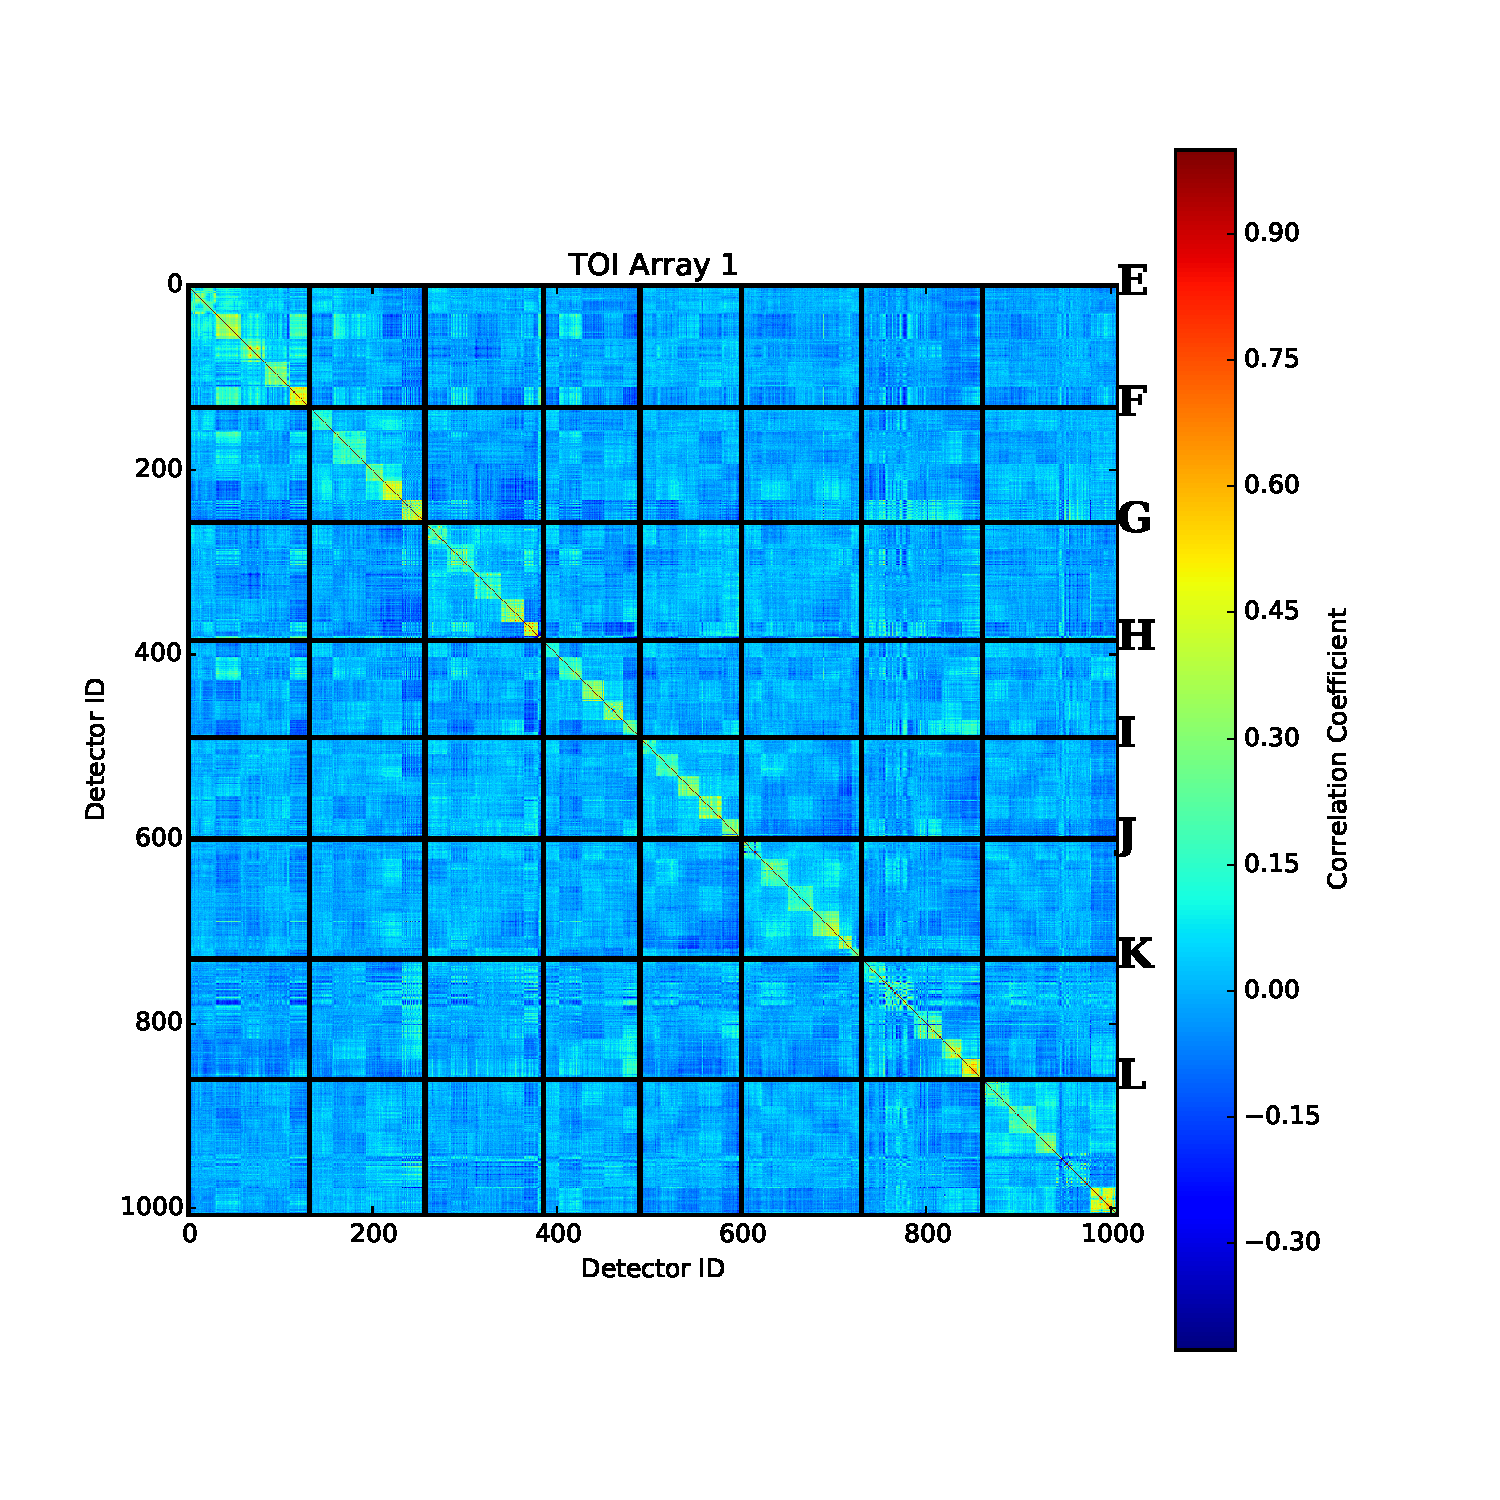
\includegraphics[width=0.3\textwidth]{Figures/NoiseTests/corrmat_TOI_PCA_array_1_20170228s151.pdf}
%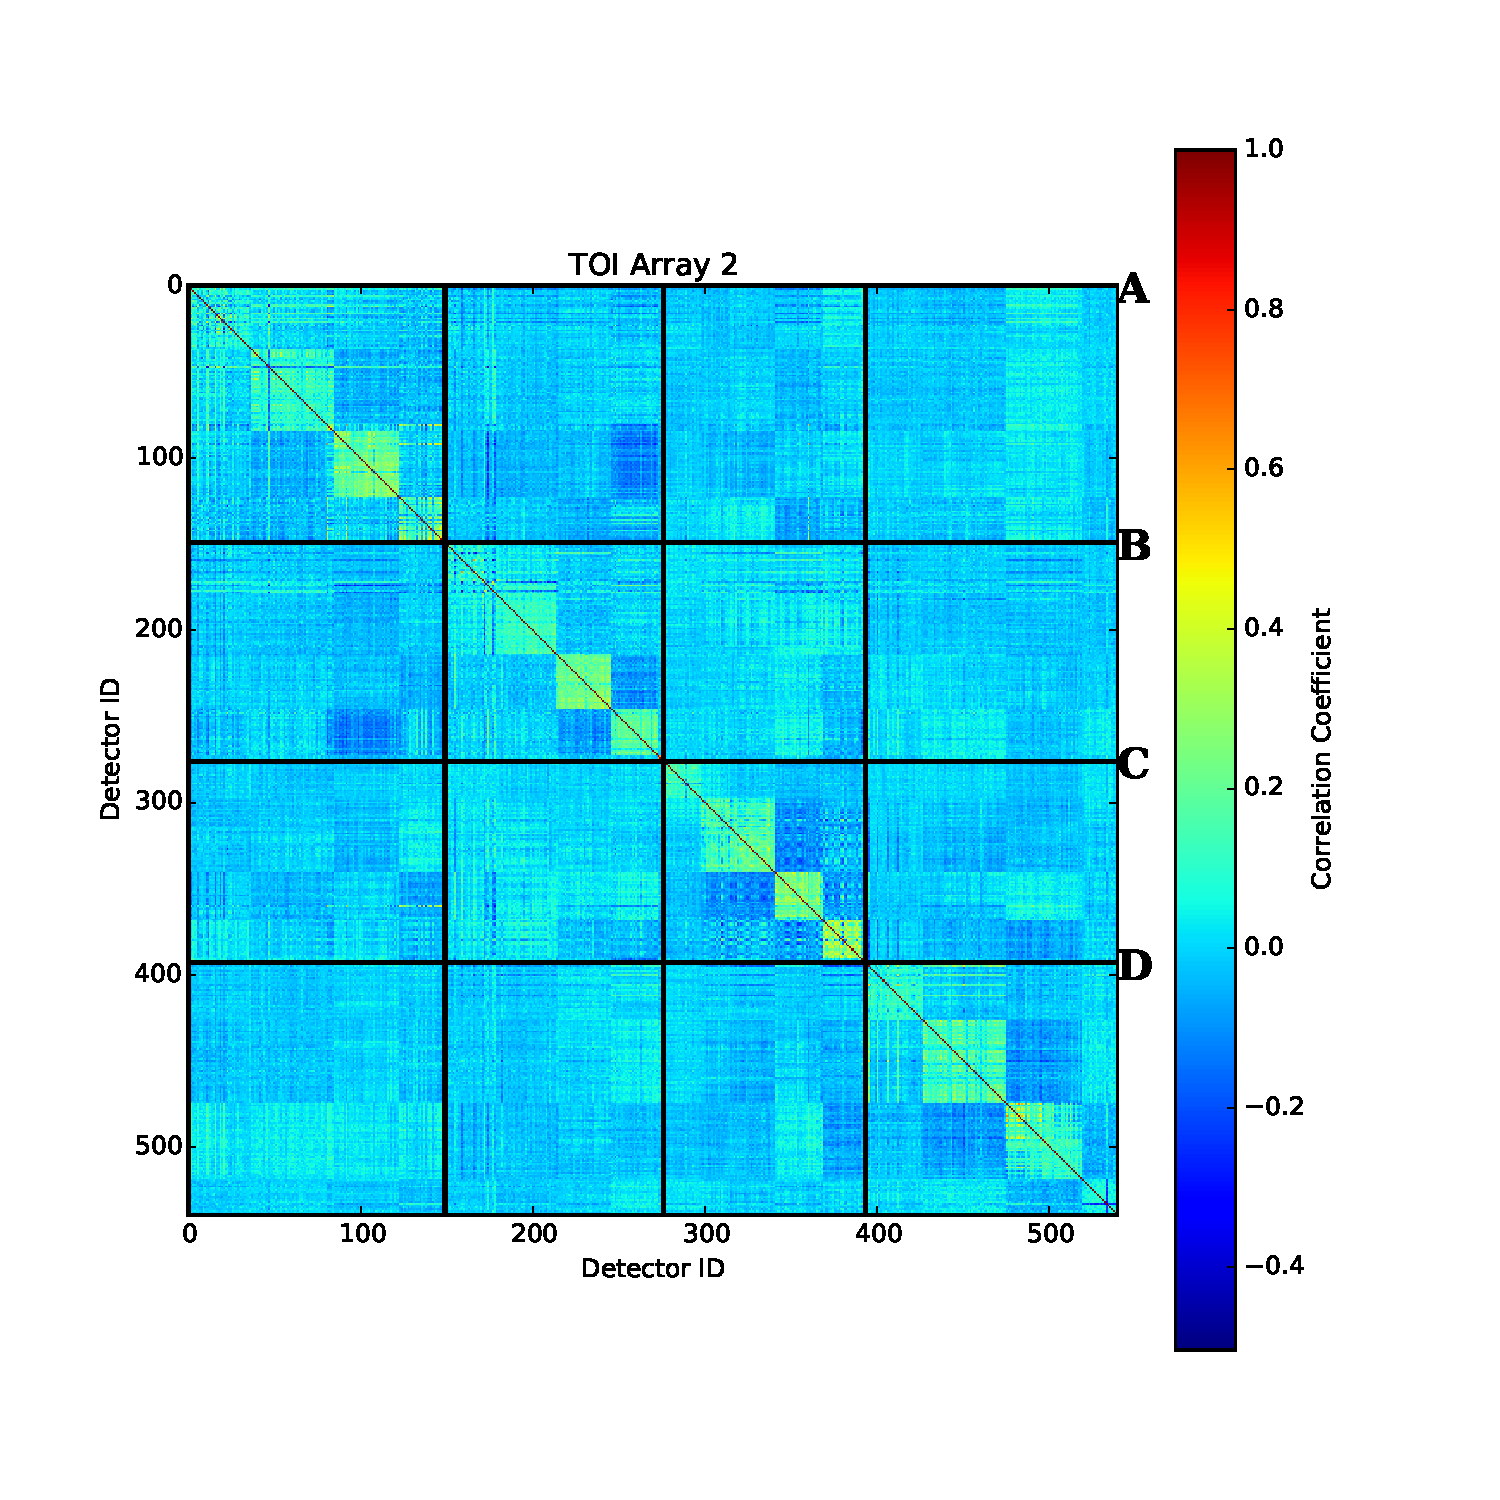
\includegraphics[width=0.3\textwidth]{Figures/NoiseTests/corrmat_TOI_PCA_array_2_20170228s151.pdf}
%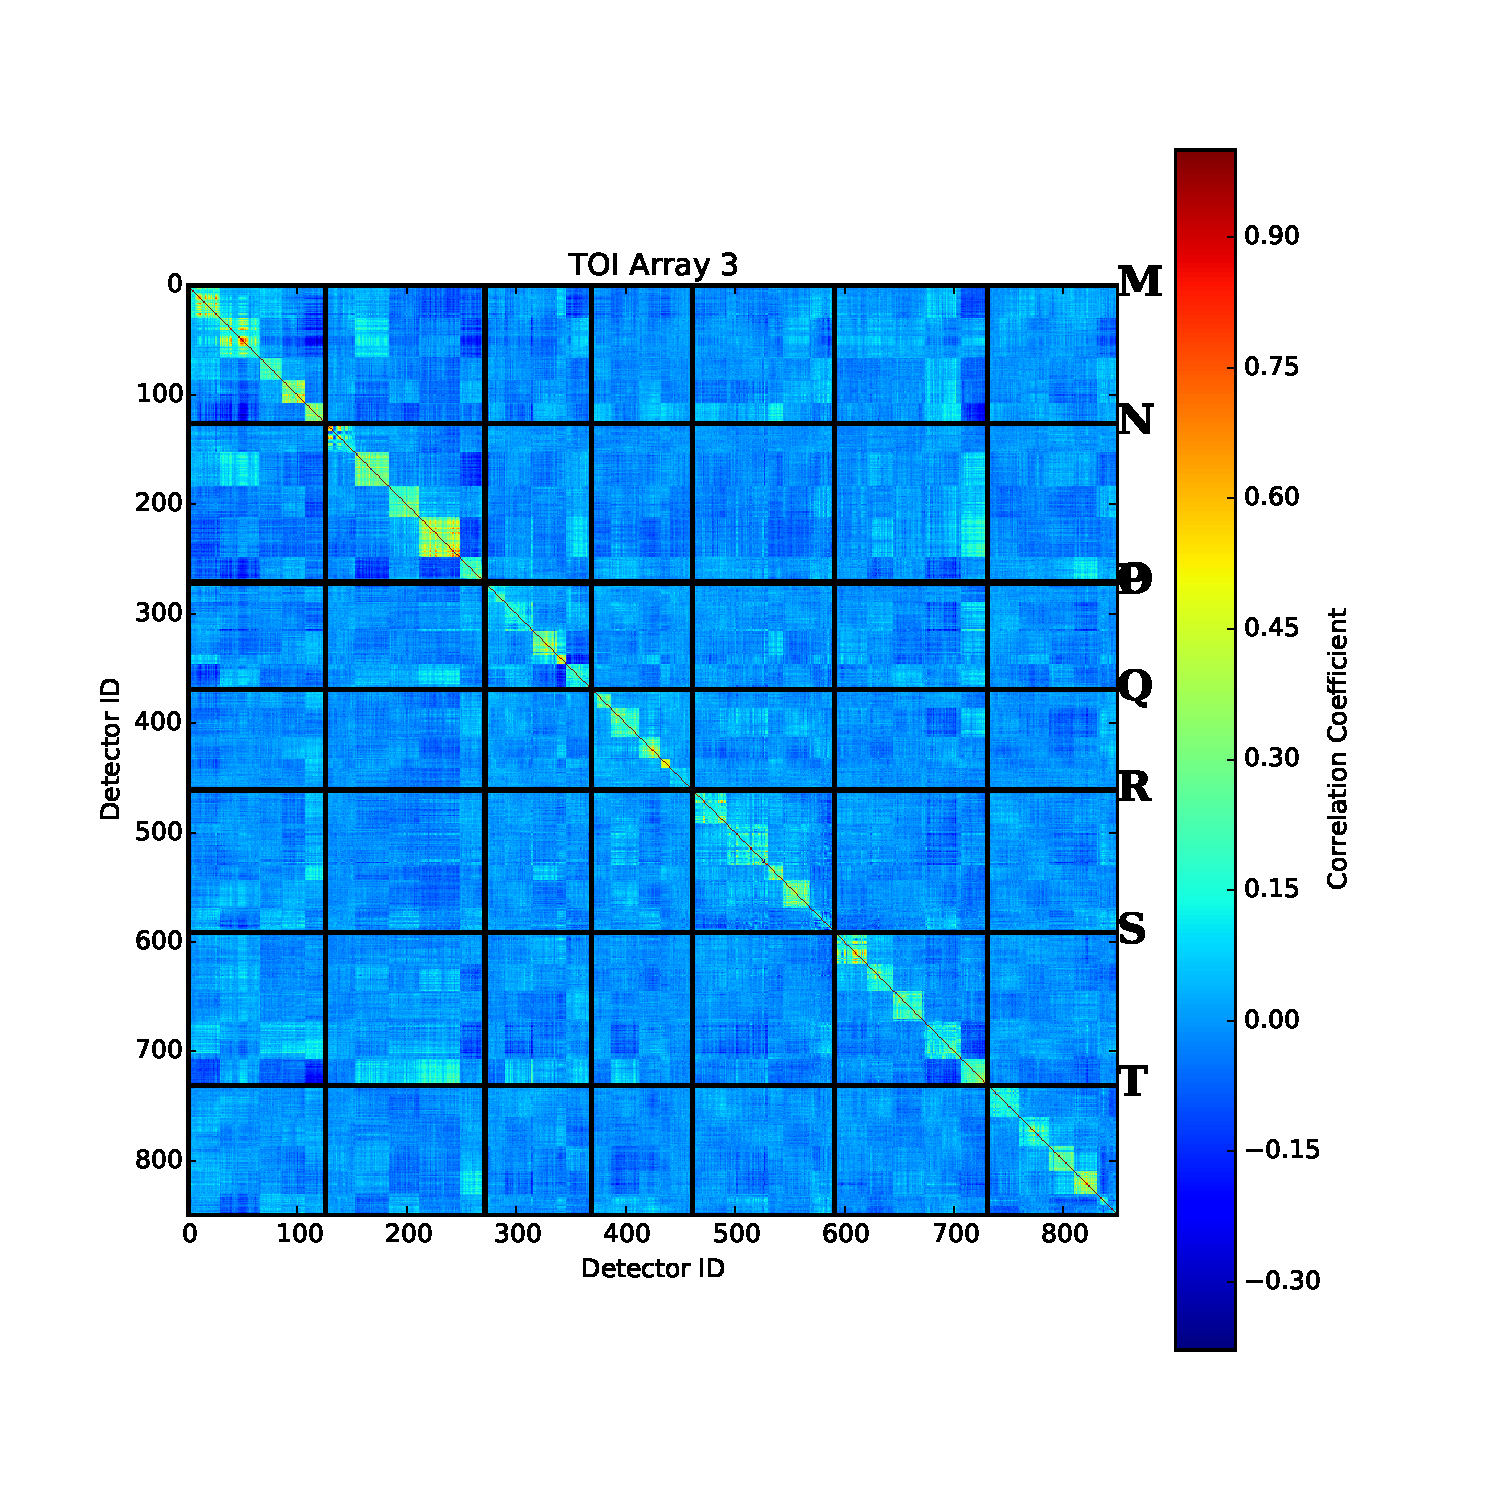
\includegraphics[width=0.3\textwidth]{Figures/NoiseTests/corrmat_TOI_PCA_array_3_20170228s151.pdf}
%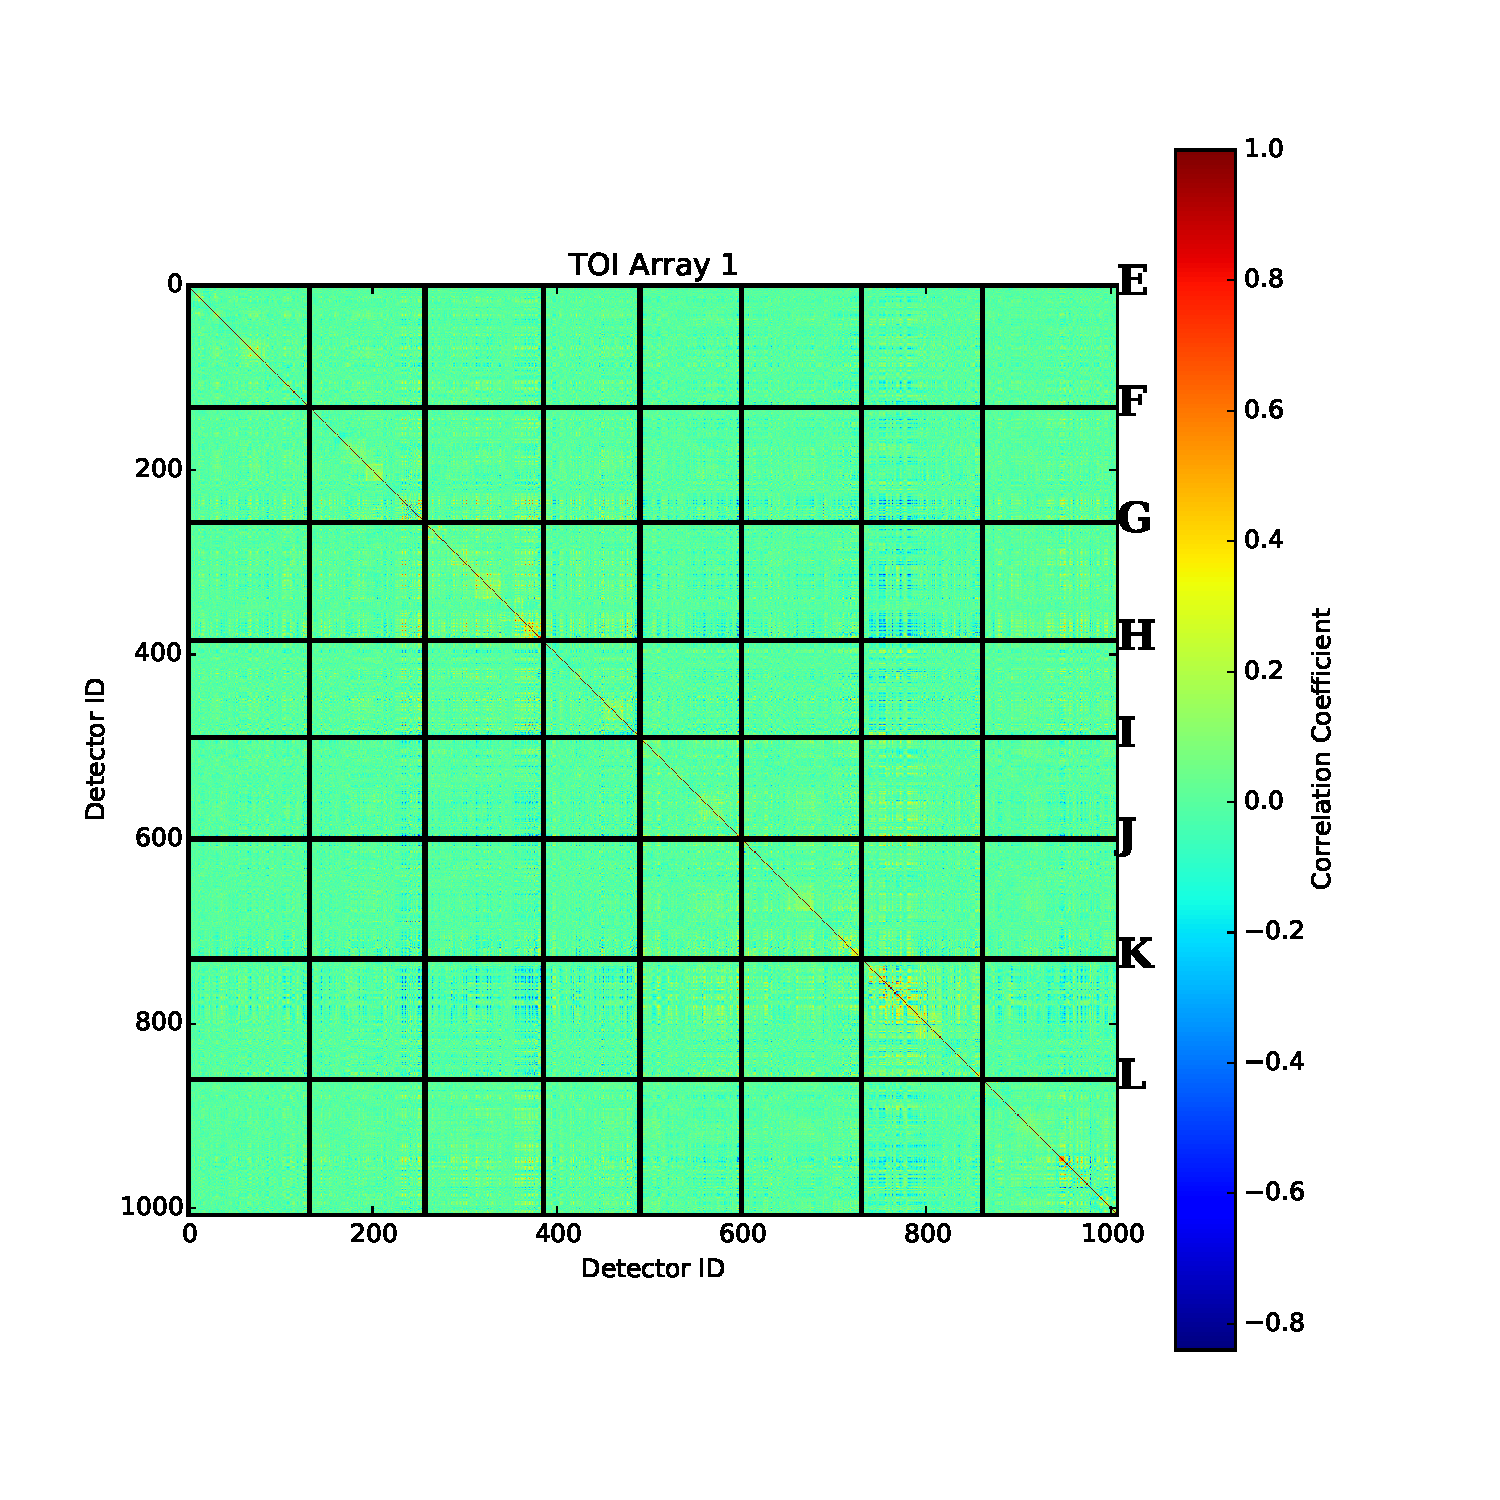
\includegraphics[width=0.3\textwidth]{Figures/NoiseTests/corrmat_TOI_BCP_array_1_20170228s151.pdf}
%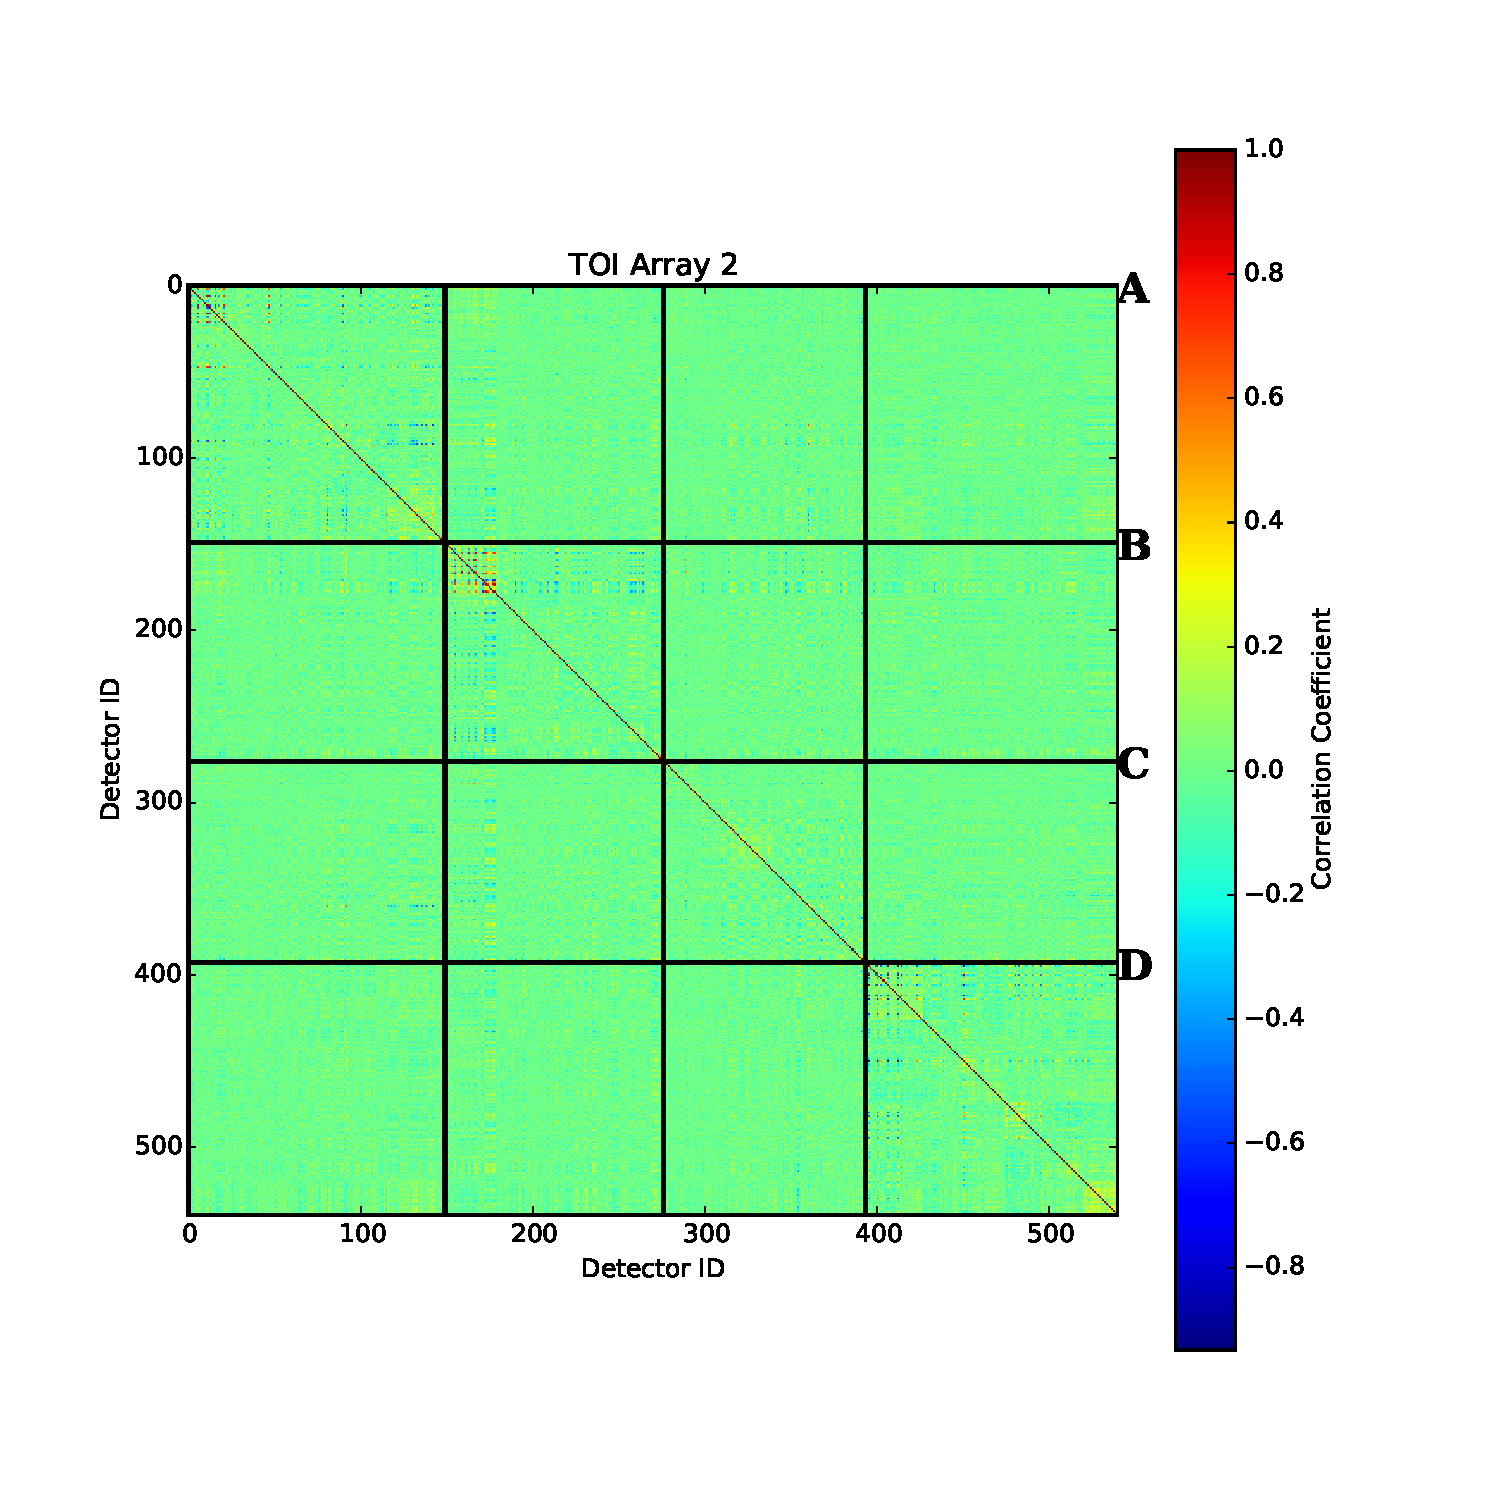
\includegraphics[width=0.3\textwidth]{Figures/NoiseTests/corrmat_TOI_BCP_array_2_20170228s151.pdf}
%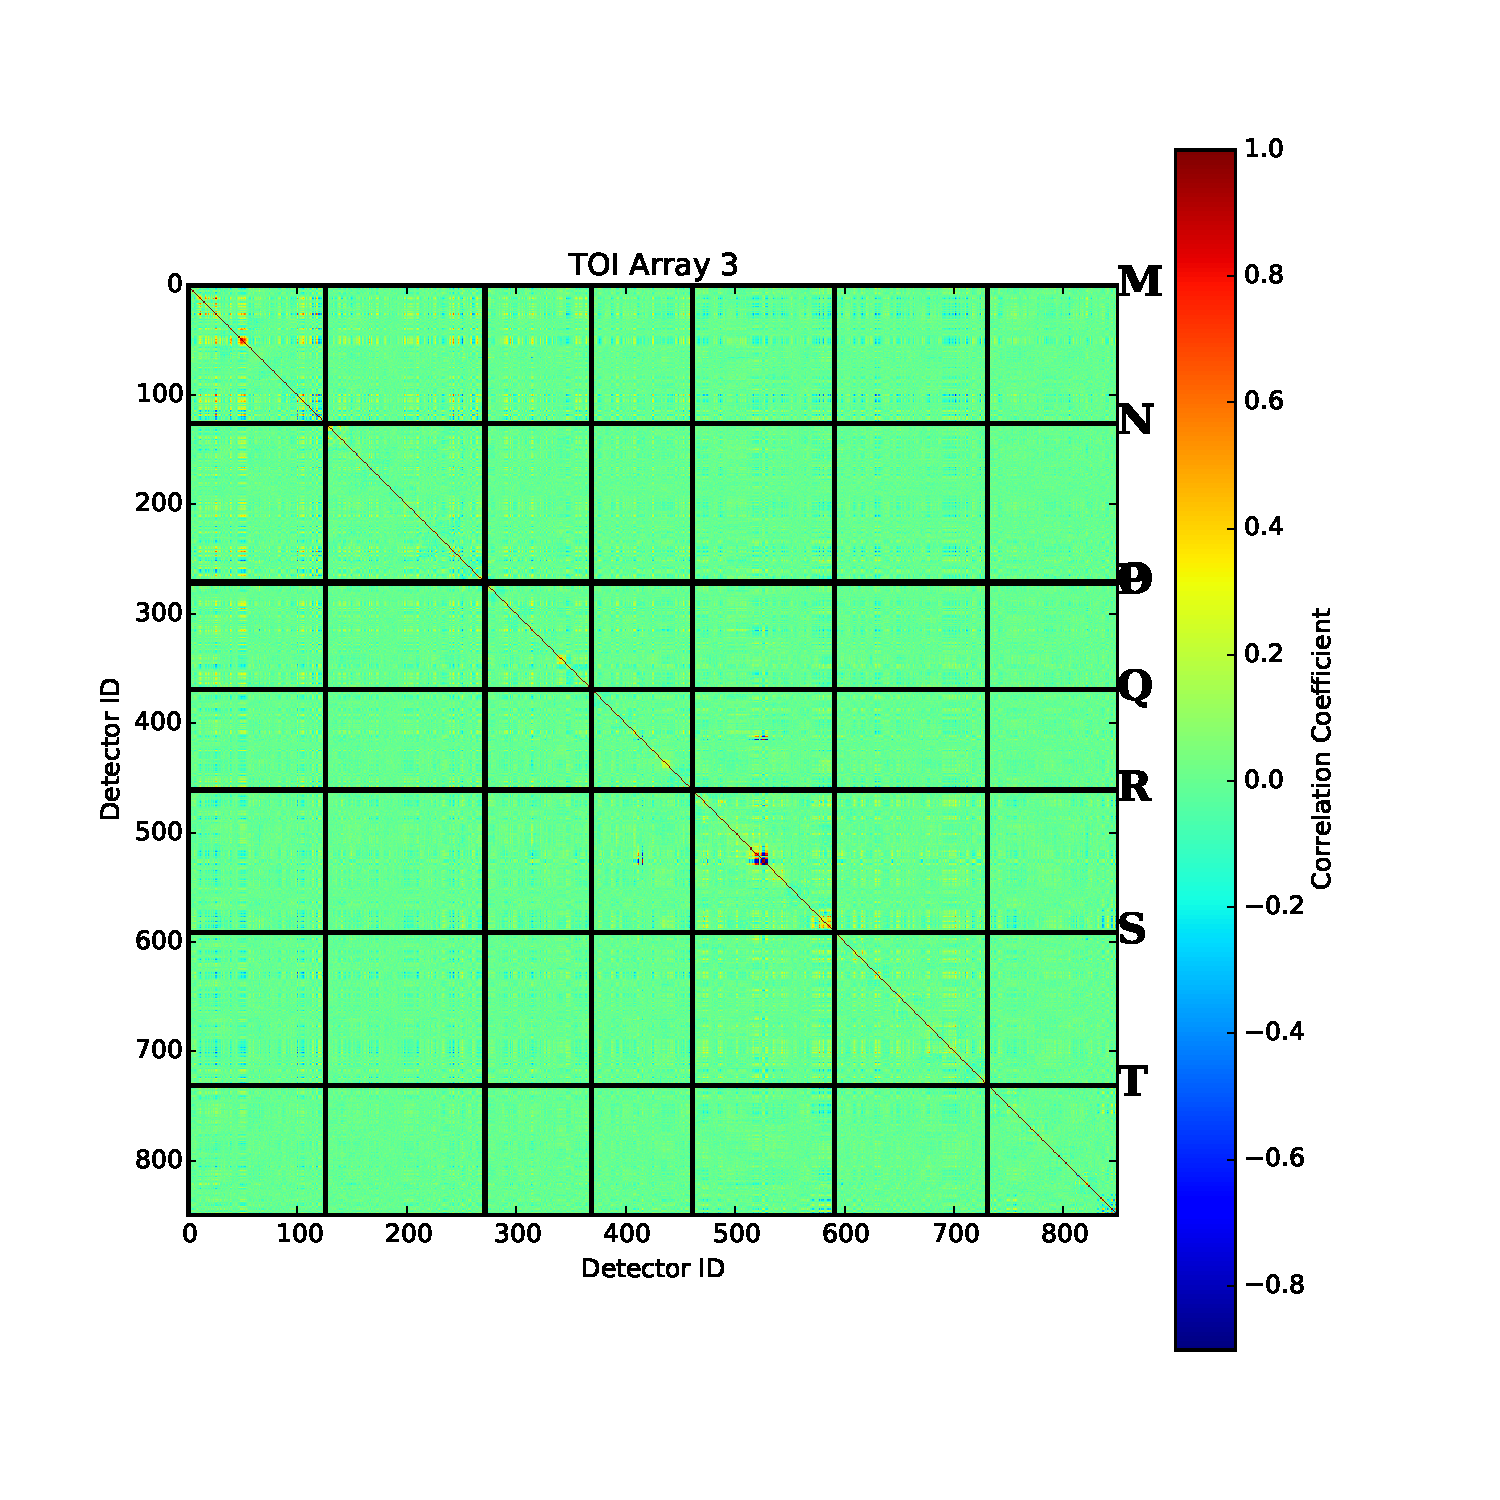
\includegraphics[width=0.3\textwidth]{Figures/NoiseTests/corrmat_TOI_BCP_array_3_20170228s151.pdf}
%\end{center}
%\caption[KID-to-KID correlation matrices]{\emph{From left to right:} TOI correlation
%  matrices for the three NIKA2 arrays (A1, A2, and A3) for scan
%  20170228s150. From top to bottom we present the correlation of the raw data,
%  after CM, PCA and MCP decorrelation methods. \label{corrmatrix}}
%\end{figure}
%
%As presented on Fig.~\ref{fig:nika_toi}, the atmosphere and the electronic noise
%combine into a large low frequency component that we want to eliminate as much
%as possible. Most of the atmospheric component is common to all KIDs, which is
%expected because the telescope is a $30\,\rm{m}$ dish and therefore
%has a near field limit at 900\,km.

As illustrated on the upper panel of Fig.~\ref{fig:nika_toi}, the
low-frequency noise component is seen by all KIDs at the same time,
while the astrophysical signal {\lp (Uranus in this case)} is shifted
from one KID to another.
{\lp In this figure the KID TOIs have been rescaled to be null
at $t=0$.} 
A simple average of the KID TOIs provides an
estimate of the low-frequency noise component, that we referred to as
a \emph{common mode}, while the signal is averaged out. The common
mode shown as a red line on the lower panel of
Fig.~\ref{fig:nika_toi}, is then subtracted to each KID TOI.

%On Fig.~\ref{fig:nika_toi}, the planet Uranus is visible in the TOIs and serves as
%guide to both the noise relative amplitude and the discussion about TOI
%processing in the following.

%On Fig.~\ref{corrmatrix}, we take a scan on Pluto
%where the signal is negligible compared to noise on the timescale of a scan to
%focus on the noise properties. We present the KID to KID timeline correlation
%matrices for the three arrays,

%In Fig.~\ref{rmspws} we present the noise power spectra of
%a typical datastream, 
%either before any data reduction or with
%different estimates of the low frequency component:

%\begin{itemize}
%\item {\bf Common Mode decorrelation (CM)}. We use all detectors of the same
%  array to build an average low frequency component nicknamed \emph{common
%    mode}. This mode is then linearly regressed and subtracted from each KID
%  timeline. In this method, the \emph{common mode} at time $t$ is the median of
%  all KIDs at this time $t$.
%
%\item {\bf Principal Component Analysis (PCA)}. For each NIKA2 array
%  independently we decompose the covariance matrix in principal components. From
%  those we derive up to 10 independent templates corresponding to the largest
%  eigenvalues that we subtract from the TOIs.
%
%\item {\bf Most correlated pixels (\cmoneb)}. For each detector in a given array we
%  identify the detectors that are most correlated to it (a minimum of
%  15). Using those detectors we compute a common mode like in method CM but with
%  more refinements to be valid even on bright sources (see below).
%\end{itemize}

% We observe that after decorrelation we reduce significantly the rms of the
%noise. Equivalently, the $1/f$-like noise in the power spectra
%(principally due to atmospheric emission)
%is significantly reduced leading to nearly flat spectra down to 0.05 Hz, with
%larger $1/f$-like residual noise for the CM decorrelation method at lower
%frequencies. This is translated into a larger rms noise for this method with
%respect to the others. For the three arrays we find increasing noise with
%increasing resonant frequency within each electronic box. This is probably
%related to the difference of gains between subbands in the readout
%electronics. %We also find for the three arrays some noise bursts that are not
%fully consistent from one decorrelation method to another. 

%Studies of the KID to KID timeline correlation matrices
%As expected the raw data noise correlation is dominated by atmospheric
%noise and we observe full correlation between detectors but for badly
%behaving detectors which are removed from the analysis.
%Significant residual correlation and anti-correlation is
%observed after CM decorrelation. This is both due to spatial changes in the
%atmospheric emission (overall residuals) and to instrumental and electronic
%noise characteristics (correlation blocks that can be associated to electronic
%boxes).  The PCA decorrelation leads to approximately block-diagonal correlation
%matrices. These observed blocks in the correlation matrix can be associated to
%first order to the different sub-bands in each of the electronic boxes. In the
%case of the MCP decorrelation, for which only those pixels highly correlated to
%the pixel of interest are used, we observe that the correlation matrix is more
%diagonal than in the two other derivations of the common mode.

\begin{figure}[ht!] % Inline image example
  \begin{center}
    % A1
%    \begin{overpic}[clip=true, trim={0.5cm, 0, 0, 0.6cm},width=0.59\textwidth]{Figures/NoiseTests/rms_TOI_array_1_20170228s151_mod.pdf}
%      \put(3,5){\rotatebox{90}{\scriptsize Noise RMS [arbitrary units]}}
%  \end{overpic}
    \begin{overpic}[clip=true, trim={0.5cm, 0, 0, 0.5cm},width=0.40\textwidth]{Figures/pws_TOI_array_1_20170228s151_mod.pdf}
      \put(2,15){\rotatebox{90}{\scriptsize P$_{\nu}$ [arbitrary units]}}
  \end{overpic}
% A3
%    \begin{overpic}[clip=true, trim={0.5cm, 0, 0, 0.5cm},width=0.59\textwidth]{Figures/NoiseTests/rms_TOI_array_3_20170228s151_mod.pdf}
%      \put(3,5){\rotatebox{90}{\scriptsize Noise RMS [arbitrary units]}}
%    \end{overpic}
    \begin{overpic}[clip=true, trim={0.5cm, 0, 0, 0.5cm},width=0.40\textwidth]{Figures/pws_TOI_array_3_20170228s151_mod.pdf}
      \put(2,15){\rotatebox{90}{\scriptsize P$_{\nu}$ [arbitrary units]}}
    \end{overpic}
    % A2
%    \begin{overpic}[clip=true, trim={0.5cm, 0, 0, 0.6cm},width=0.59\textwidth]{Figures/NoiseTests/rms_TOI_array_2_20170228s151_mod.pdf}
%      \put(3,5){\rotatebox{90}{\scriptsize Noise RMS [arbitrary units]}}
%    \end{overpic}
    \begin{overpic}[clip=true, trim={0.5cm, 0, 0, 0.5cm},width=0.40\textwidth]{Figures/pws_TOI_array_2_20170228s151_mod.pdf}
      \put(2,15){\rotatebox{90}{\scriptsize P$_{\nu}$ [arbitrary units]}}
    \end{overpic}
  \end{center}
\caption[Noise power spectra]{
  The data noise power spectra are shown for the three NIKA2 arrays (A1, A3, and
  A2 from top to bottom). % for scan 20170228s151.
  The power spectra are given for the raw
  data (blue), and for noise decorrelated data using the common mode
  (labeled CM, green), the PCA (red) and the \cmoneb\ (labeled MCP,
  cyan) methods.
  \label{rmspws}}
\end{figure}

{\lp For the calibration and performance assessment, we use an
atmospheric and electronic noise
decorrelation method named \cmoneb\, which comprises two
additional technicalities with respect to the common mode
method.} First, the signal contamination of the common mode estimate
is mitigated by discarding on-source KID data samples before averaging
the rescaled TOI. Second, instead of a single common mode subtraction to
all KIDs, we estimate an accurate common mode for each
KID. Calculating the KID-to-KID cross-correlation matrix, we
identify the most correlated KIDs. Then, we build an
inverse noise weighted co-addition of the timelines of the %off-source
KIDs that are the most correlated with the KID under
concern. Furthermore, we have tested on simulations that this method
does preserves the flux of {\lp point-like or moderately extended sources.}
% Regarding very extended sources (over more
%than a few arcminutes), the noise decorrelation requires iterative or
%more evolved methods, as will be discussed in \citet{Ponthieu2019}.}

In Fig.~\ref{rmspws} we present the noise power spectra of
a typical KID TOI both before any data reduction and using three noise
decorrelation methods, which are the simple common mode (CM) method
used in Fig.~\ref{fig:nika_toi}, a method based on a principal component
analysis (PCA) and the \cmoneb\ method (MCP). We observe that after decorrelation the
$1/f$-like noise in the power spectra (principally due to atmospheric
emission drifts)
is significantly reduced leading to nearly flat spectra down to {\lp 0.5~Hz}, with
lower $1/f$-like residual noise for the PCA and the \cmoneb\ methods
than the common mode decorrelation at low frequencies. {\lp Moreover, we
have checked using simulations that the \cmoneb\ method was more
efficient than the PCA in preserving the astrophysical signal. The
former is thus preferred over the latter.} 

%We have investigated several ways of using this information to remove this
%component from the TOIs. Our prefered choice so far, that is the reference
%method for this document, is the \cmoneb\ method, that we describe into further
%details below:
%
%\begin{itemize}
%\item From the pointing information (Sect.~\ref{se:ptg}), we derive a mask per TOI
%  and for each time $t$ that is 0 if the KID is close to the source, 1
%  otherwise. In the case of a point source, the mask consists in 
%    a radius of 60\,arcsec centered on the source, whereas for
%    diffuse emission, tailored masks are build.
%\item Only samples for which two KIDs are far from the source,
%  hence which are not discarded using the mask, are selected and the KID-to-KID
%  correlation is computed.
%\item For a KID $k_0$, we store the KID identifiers that are most
%  correlated to it. We first select the 15 most correlated KIDs, then 
%  the average and the dispersion $\sigma$ of these correlations are
%  computed. Then we add to the selection all the KIDs that are as correlated to $k_0$ as the
%  15 first, up to $2\,\sigma$.
%\item A median common mode (far from the source) for this block of 15
%  or more KIDs is derived.
%\item A cross-calibration to each of these KIDs is computed using the
%  median common mode. Then an inverse noise weighted average mode is build. At each time, we use
%  only KIDs that are not discarded with the source mask.
%  At this stage it is important to verify to have enough KIDs to produce a
%  continuous mode and to do not leave samples without any estimation.
%\item We linearly regress this average mode against $k_0$'s TOI (far from the
%  source) and subtract on the entire $k_0$ timeline.
%\end{itemize}
%
%This process is repeated for each KID. Fig.~\ref{fig:nika_toi} shows an example
%of this low frequency mode derivation, together with the resulting TOI
%cross-correlation matrix after its subtraction. We have tested on simulations
%that this method does not alter the flux of the
%source.
%
%If the observed field contains something else than a single point source at its
%center, then several options are available to generalize this method. In
%particular, the mask can be designed to adjust to several point sources. If the
%source is diffuse and extended, then we may go through an iterative procedure that
%subtracts an improved derivation of the signal at each step. For this work about
%the commissioning of the instrument and the assessment of its performances on
%point sources, we do not need to go into further details about this.\\

%We now focus on the absolute calibration of each TOI. As stated in
%Sect.~\ref{se:ll_proc}, at this stage of the reduction each KID \rf~timeline is
%in Hz. The conversion process to go from these Hz into Jy/beam proceeds in two
%steps: a standard absolute calibration and a correction for the current opacity
%and elevation.
%
%The standard conversion from Hz to Jy/beam is stored in the
%\kidpar\ database. The derivation of these gains $g(k)$ is detailed in
%Sect.~\ref{se:geometry}. Suffice is to say here that simply multiplying
%the TOI's by these gains converts them into Jy/beam. Of course, this individual
%absolute calibration also acts as a relative calibration. This calibration is
%meant to work at zero opacity and 90$^\circ$ elevation. We thus need to correct
%for the current opacity $\tau$ and elevation. In short, the absolute calibration reads
%
%\begin{equation}
%TOI^k(t) [{\rm Jy/beam}] = \rf^k(t)[{\rm Hz}] \times g(k) \times e^{\tau_t/\sin\elev_t}
%\end{equation}
%
%The derivation of opacity is presented in Sect.~\ref{se:opacity}. \\

%\noindent \emph{Map projection.}
\subsection{Map projection}
\label{se:map_projection}
We use the pointing information to project the cleaned (low-frequency
noise subtracted) calibrated TOI of all the valid KIDs of an array
onto a flux density map (tangential projection). This map $M_p$ is produced using an inverse
variance noise weighting of all of the data samples that fall into a map
pixel as defined using a nearest grid point scheme. We also compute
the associated count map $H_p$ defined as the number of data samples
per map pixels. The map resolution
is chosen small enough (typically $2''$ per map pixel) to alleviate
the need for more refined interpolation scheme. The noise variance
$\sigma_k$ for each KID $k$ is evaluated by the standard deviation of the
KID TOI far from the source position. 
%nk_w8.pro in nk_scan_reduce.pro
%nk_projection_4.pro
%%%%%%%%%%%%%%%%%%%%%%%%%%%%%%%%%%%%%%%%%%%%%%%%%%%%%%%%%%%%%%%%%%%%%%%
{\lp The variance map $\sigma_p^2$ is inhomogeneous and varies as the
inverse of $H_p$. Its normalisation is evaluated using the
homogeneous background map variance, that is the
variance of $M_p\sqrt{H_p}$ calculated far from the source.}
%nk_bg_var_map
%%%%%%%%%%%%%%%%%%%%%%%%%%%%%%%%%%%%%%%%%%%%%%%%%%%%%%%%%%%%%%%%%%%%%%%%
%{\lp If the noise was white and uncorrelated from KID to KID, this
%inverse variance noise weighting of the data samples would produce an
%optimal flux density map $M_p$ with variance
%\begin{equation}
% \sigma^2_p = \left( \sum_{k}(A_{pt}^k)^{t} 1/\sigma_k^2 A_{pt}^k \right)^{-1},
%\end{equation}
%where $A^k$ is the pointing matrix for the KID $k$ that selects all the
%data samples $t$ falling into the map pixel $p$~\citep{Tegmark1997}.}
%\begin{equation}
% \sigma^2_p = \left( \sum_{k, \, t\, \in p}\, 1/\sigma_k^2 \right)^{-1},
%\end{equation}
%where the sum is performed over all KIDs $k$ and all data samples $t$
%falling into the map pixel $p$~\citep{Tegmark1997}.}

%We neglect the KID-to-KID correlated noise residuals in this
%procedure.
%This is due to the remaining correlations between TOIs before projection. At this stage,
%rather than putting more effort in TOI processing, we renormalize the width of
%the Gaussian noise, which actually increases the map variance by the required factor
%so that the SNR distribution becomes normalized. This normalization factor
%varies from scan to scan but it is usually between 1.2 and 1.5. It is estimated on
%the background of the map, i.~e. far from the source.

{\lp To account for the residual
correlated noise while evaluating the variance map, we resort to an
effective approach.
First, we compute the map of the signal-to-noise ratio (SNR) as the ratio of
$M_p$ and the noise map $\sigma_p$, that is the square root of the
variance map. We observe that the distribution of the SNR map over the pixels far from the source is
well-approximated with a Gaussian but has a width larger than the
expected unity. This is due to the remaining correlations between KID TOIs
before projection. Then, we multiply the noise map 
$\sigma_p$ by the required factor so
that the width of SNR distribution becomes normalized.
%Then, we normalise the SNR distribution by
%increasing the noise variance by a factor that goes from 1.2 to 1.5.
This normalizing factor ranges from 1.2 to 1.5 depending on the observing conditions. This
constitutes an effective approach to account for the pixel-to-pixel
correlation matrix off-diagonal terms alleviating the need of
accurately measure them.}
%This constitutes an effective approach to account for
%the correlated noise residuals in the map. 
%to correct
%for the KID-to-KID correlation matrix off-diagonal terms alleviating
%the need of accurately measure them. 

%At this stage, data have been calibrated and cleaned and we have the pointing
%information for each sample. If the noise was white and uncorrelated from KID to
%KID, we would be able to produce an optimal map $S_p$ using an inverse
%variance noise weighting of all of the measurements $m^k_t$ that fall
%into a map pixel $p$ with a simple Nearest Grid Point procedure. In
%this scheme, data samples are coadded with inverse variance noise
%weighting: for each KID, we compute the standard deviation
%$\sigma_k$ of its TOI far from the source (see Sect.~\ref{se:toi_proc}). Each
%sample of this KID therefore has a weight of $1/\sigma_k^2$ and
%
%\begin{eqnarray}
%S_p        &=& \frac{1}{\sum_{k,t}1/\sigma_k^2}\sum_{k,t} \frac{m^k_t}{\sigma_k^2}\,, \label{eq:ngp_sum}\\
%\sigma^2_p &=& \sum_{k,t}1/\sigma_k^2\,, \label{eq:ngp_var}
%\end{eqnarray}
%
%where $\sigma^2_p$ is the variance associated to pixel $p$. The
%pipeline automatically projects one map per array and a combined 1\,mm
%map and takes a small enough resolution to respect the Nyquist
%criterion on the beam sampling.
%To keep margin
%and for the sake of simplicity, we usually take 2\,arcsec resolution pixels.

%In practice, and although the data cleaning procedure described in
%Sect.~\ref{se:toi_proc} significantly reduces the low frequency component of
%TOIs, the residual noise is still not completely white nor KID independent. The
%correlation matrix is not strictly zero to begin with (Fig.~\ref{fig:nika_toi})
%and when looking at the distribution of the SNR on maps and variance maps
%obtained with Eqs~(\ref{eq:ngp_sum},\ref{eq:ngp_var}), the distribution is
%Gaussian, but not normalized to unity. %(see
%Fig.~\ref{fig:sigma_boost}).
%This is due to the remaining correlations between TOIs before projection. At this stage,
%rather than putting more effort in TOI processing, we renormalize the width of
%the Gaussian noise, which actually increases the map variance by the required factor
%so that the SNR distribution becomes normalized. This normalization factor
%varies from scan to scan but it is usually between 1.2 and 1.5. It is estimated on
%the background of the map, i.~e. far from the source.

%\begin{figure}[ht!]
%\begin{center}
%\includegraphics[clip, angle=0, scale=1, width=0.75\textwidth]{Figures/sigma_boost.eps}
%\caption[Distribution of the SNR per beam]{Histogram of the SNR per beam on a scan of weak source (G2, see
%  Sect.~\ref{se:nefd_estimation_methods}). While the histogram is Gaussian, its
%  width is not normalized to 1 due to residual correlated noise between the
%  TOIs. This factor is accounted for before delivering the final variance map
%  and associated flux estimates.}
%\label{fig:sigma_boost}
%\end{center}
%\end{figure}

When several scans of the same source are averaged, we apply an inverse
variance weighting as well. %Weights are taken from the variance maps of each scan,
%corrected for the excess variance mentioned in the previous
%paragraph.
The variance map of the sum of scans is also corrected to ensure unity-width
SNR distribution.


%%%%%%%%%%%%%%%%%%%%%%%%%%%%%%%%%%%%%%%%%%%%%%%%%%%%%%%%%%%%%%%%%%%%%%%%%%%
% photometry
% nk_save_scan_results_3 -> nk_grid2info -> nk_map_photometry
%%%%%%%%%%%%%%%%%%%%%%%%%%%%%%%%%%%%%%%%%%%%%%%%%%%%%%%%%%%%%%%%%%%%%%%%%%%%

%As described in Sect.~\ref{se:photometric_system}, the flux density of
%point-like sources is estimated as the amplitude of a
%fixed-width reference Gaussian fitted on the map.

%\noindent \emph{Photometry}
%\label{se:intro_photometry}

%Throughout this document, we adopt the following convention. Assuming the beam
%is a perfect Gaussian of known $FWHM=\sigma\sqrt{8\ln 2}$, the instantaneous
%signal measured by a KID is

%\begin{equation}
%m^k(x,y) = \phi e^{-(x^2+y^2)/2\sigma^2} = \phi G(x,y)
%\label{eq:flux_per_beam_def}
%\end{equation}

%with $\phi$ the flux of the source and $(x,\, y)$ the coordinates in
%the chosen system. In practice, the beam is not a perfect Gaussian
%and significant side lobes must be accounted for
%(Sect.~\ref{se:beam}). If the beam was perfectly known and stable, we could in
%principle replace the Gaussian form in Eq.~\ref{eq:flux_per_beam_def} by the
%beam pattern and fit for the amplitude $\phi$.
%In practice, we have found that
%it was enough as a first approximation to take an equivalent effective Gaussian
%width and use it to derive the beam template.
%In practice, the beam pattern i) has a complexe structure, including
%features which can rotate with the observation elevation (as presented
%in Sect.~\ref{se:fullbeam}), ii) has a few percent dispersion across the FOV (see
%Sect.~\ref{se:mainbeam}) and iii) shows some variations with the observation date
%(see Sect.~\ref{se:obsdate_variations}). However, we have found that using an equivalent
%effective fixed-width Gaussian for the photometry, as presented in
%Sect.~\ref{se:calibration}, is sufficient to ensure accurate, stable and robust flux
%measurements, as assessed in Sect.~\ref{se:photometry}. The reference fixed-width
%Gaussian is chosen sizably larger than the measured main beam width
%(see Sect.~\ref{se:mainbeam}) to account for a fraction of the
%signal stemming from the error beams and side lobes. Namely, we take
%12.5 and 18.5\,arcsec FWHM at 1 and 2\,mm respectively and compute all our fluxes with these
%values. We do this for both absolute calibrators (see Sect.~\ref{se:calibration})
%and analyzed point sources (see Sect.~\ref{se:photometry}) to be consistent. Our
%photometric system is further detailed in Sects.~(\ref{se:calibration}).

%Let's call $s_p$ the measured signal at map pixel $p$ and denote by $g_p$ the
%Gaussian weight given to pixel $p$ as a function of its distance to the source,
%as defined in Eq.~\ref{eq:flux_per_beam_def}. The amplitude fit is performed
%with an usual maximum likelihood approach. We assume that the renormalization of
%the variance map described in the previous section is enough to account for the
%residual noise correlations from pixel to pixel and therefore assume the pixels to
%be independent in this estimator:
%
%\begin{eqnarray}
%\hat{\phi} &=& \frac{1}{\sum_p g_p^2/\sigma_p^2}\sum_p
%s_p\frac{g_p}{\sigma_p^2} \label{eq:flux_estim_def} \\
%\sigma^2(\hat{\phi}) &=& \frac{1}{\sum_p
%  g_p^2/\sigma_p^2} \label{eq:flux_estim_var_def}
%\end{eqnarray}
%
%In the case of Gaussian white noise, this maximum likelihood estimator coincides
%with the classical minimum variance estimator and thus provides the best SNR
%estimate of the source flux.

%% \subsection{Opacity correction}
%% 
%% Water vapor along the line of sight absorbs power from the source and therefore
%% biases the flux measurement. At the same time, the overall airmass acts as a
%% diffuse source of power on the KIDs that induce a variation of their resonance
%% frequency. We are able to calibrate it and therefore derive the opacity in real
%% time from \nika\ data. This is described in details in
%% Sect.~\ref{se:opacities}. Suffice is here to say that after the derivation of
%% the KID offsets and their relative gains as described in
%% Sect.~\ref{se:fov_first_geometry}, one we know the opacity, we can derive an
%% absolute calibration per KID.

%% \subsection{Absolute calibration}
%% \todo{See how to talk about Planet models and repeated observations of these to derive
%% the ``final'' abs. cal for the run.}
%% 
%% %The data reduction of \nika\ cannot be done exclusively KID by KID
%% %independently. Each matrix is a filled array with more than one detector per PSF
%% %and the atmosphere together with the electronics chain act as correlated
%% %noise. We therefore have to work iteratively to improve both individual and
%% %global parameters of the detectors. In this section, we give an overview of the
%% %full data reduction that illustrates this iterative process. More details on
%% %each specific step are given in other dedicated sections.
%% 
%% \subsection{Overview of the on-sky calibration method}
%% 
%% The steps to go from raw timeline data in Hertz to calibrated data in Jansky per beam comprize:
%% \begin{itemize}
%% \item[] Opacity correction
%% \item[] Field-of-view geometry and KIDs selection
%% \item[] KID-to-KID intercalibration (flat fielding)
%% \item[] Absolute calibration  
%% \end{itemize}
%% 
%% 
%% \subsection{Data reduction summary {\color{blue} Nico}}
%% 
%% The performance assessment relies on a data reduction pipeline that consists of the following steps:
%% \begin{itemize}
%% \item[] reading of the raw timeline 
%% \item[] implementation of the calibration
%% \item[] substraction of the correlated part of the noise 
%% \item[] projection of the timeline onto maps
%% \end{itemize}

\subsection{Observation scan selection}
\label{se:data_selection}

For calibration and performance assessment, we select scans in average
observing conditions by performing mild selection cuts. These scan
cuts rely on zenith opacity estimates $\taunu$ in NIKA2 bands, as
described in Sect.~\ref{se:opacity}, on the elevation and on the
observation time of the day. We select the scans satisfying the
following criteria:
%
\begin{itemize}
\item[i)] $\tau_{\rm{A_3}} < 0.5$, where $\tau_{\rm{A_3}}$ is the $\taunu$ estimate for
  Array 3; %, corresponding to a decrease of the signal by a factor of two at $45^{o}$ of elevation;
\item[ii)] $x\, \tau_{\rm{A_3}} < 0.7$ and $\elev > 20^{o}$, where
$\elev$ is the observing elevation and $x$, the
  \airmass, which depends on the elevation as $x=(\sin{\elev})^{-1}$. This
  threshold corresponds to a decrease of the astrophysical signal by a
  factor of two;
\item[iii)] observation time from 22:00 to 9:00 UT and from 10:00 to
  15:00 UT, that excludes the sunrise period and the late afternoon.
\end{itemize}
%
{\lp In the following sections, these selection cuts are referred to as the 
'\emph{baseline} scan selection'.}  
As discussed in Sect.~\ref{se:beam_variation}, the late afternoon
observations are often affected by time-variable broadening of the
telescope beams caused by (partial) solar irradiation of the primary
mirror and/or anomalous atmospheric refraction.
Around sunrise, the focus shifts continuously due to the ambient temperature
change until the temperature stabilizes, so that the scans taken from
9:00 to 10:00 UT are likely not to be optimally focused.
After the focus stabilisation, the middle of the day period ranging
from 10:00 to 15:00 UT offers stable observing conditions
provided that the telescope is not pointed too
close to the Sun.
Otherwise, further scan selection based on
the exact sequence of observations and on beam monitoring might be
needed before using these observations for performance assessment.
{\lp In summary, the \emph{baseline} scan selection retains 16 hours of
observations a day and discards observations affected by an
atmospheric absorption exceeding 100\%.}  

